\documentclass[10pt]{beamer}

\usetheme{metropolis}
\usepackage{appendixnumberbeamer}

\usepackage{booktabs}
\usepackage[scale=2]{ccicons}
\usepackage{graphicx}
\usepackage{hyperref}
\usepackage{circuitikz}
\usepackage{pdflscape}
\usepackage{smartdiagram}

\usepackage{color}
\usepackage{listings}

\lstset{
	basicstyle=\footnotesize\ttfamily,
    keepspaces=true,
    showstringspaces=false,
    language=PHP,
    commentstyle=\ttfamily,
}

\usepackage[OT4]{polski}
\usepackage[utf8]{inputenc}

\usepackage{pgfplots}
\usepgfplotslibrary{dateplot}

\usepackage{xspace}
\newcommand{\themename}{\textbf{\textsc{metropolis}}\xspace}

\setbeamertemplate{frame footer}{}
\setbeamertemplate{frame numbering}{}

\usetikzlibrary{shapes,arrows}

\tikzstyle{decision} = [diamond, draw, fill=blue!20, 
    text width=4.5em, text badly centered, node distance=3cm, inner sep=0pt]
\tikzstyle{block} = [rectangle, draw, fill=blue!20, 
    text width=5em, text centered, rounded corners, minimum height=4em]
\tikzstyle{line} = [draw, -latex']
\tikzstyle{cloud} = [draw, ellipse,fill=red!20, node distance=3cm,
    minimum height=2em]


\title{Czysty kod, część II}

\subtitle{Projektowanie i programowanie systemów internetowych I}
\author{mgr inż. Krzysztof Rewak}
\date{\today}
\institute{Wydział Nauk Technicznych i Ekonomicznych \\ Państwowa Wyższa Szkoła Zawodowa im. Witelona w Legnicy}

\begin{document}

\maketitle

\begin{frame}{Plan prezentacji}
  \setbeamertemplate{section in toc}[sections numbered]
  \tableofcontents[hideallsubsections]
\end{frame}


\begin{frame}{Czysty kod}
	\emph{Dlaczego dobry kod tak szybko się psuje?}
\end{frame}

\begin{frame}{Czysty kod}
	\emph{Wyobraźmy sobie następującą sytuację: przed operacją pacjent zdecydowanie żąda, aby lekarz przestał wreszcie myć ręce, ponieważ zabiera to zbyt wiele czasu}
\end{frame}

\begin{frame}{Czysty kod}
	\emph{Wyobraźmy sobie następującą sytuację: przed operacją pacjent zdecydowanie żąda, aby lekarz przestał wreszcie myć ręce, ponieważ zabiera to zbyt wiele czasu.}
\end{frame}

\begin{frame}{Czysty kod}
	\emph{Skauci amerykańscy mieli prostą zasadę, jaką można zastosować w naszym zawodzie:}
	
	\emph{Pozostaw obóz czyściejszym, niż go zastałeś.}
\end{frame}

\section{Funkcje}

\begin{frame}{Funkcje}
	Funkcja czy metoda to podstawowa jednostka operacyjna w naszych programach.
\end{frame}

\begin{frame}{Funkcje}
	Zatem warto przede wszystkim zachować porządek w samej budowie funkcji.
	
	Niektóre języki są dosyć liberalne pod względem definiowania argumentów czy zwracanych typów, ale nie powinniśmy nadużywać tej możliwości.
\end{frame}

\begin{frame}
	\begin{figure} \centering
		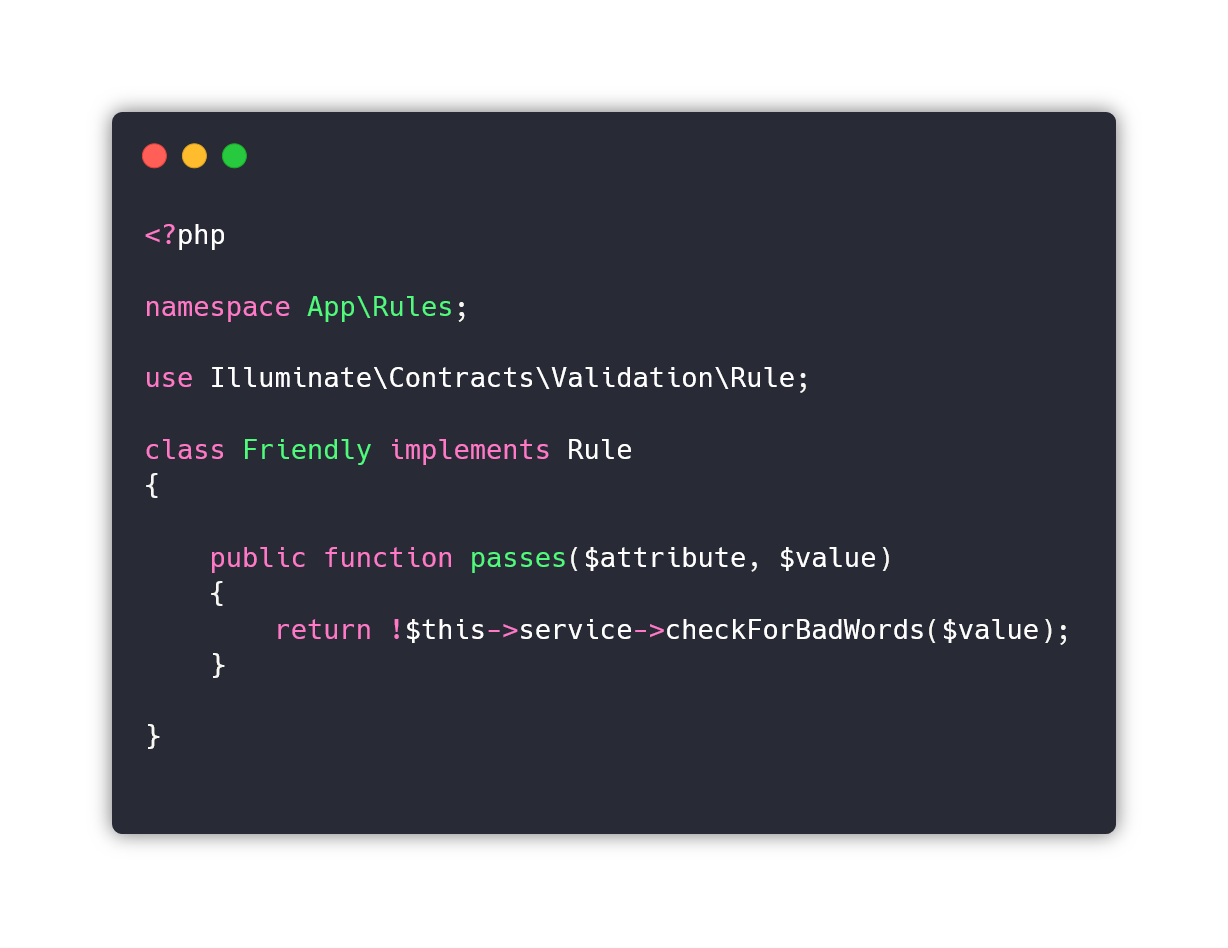
\includegraphics[width=\textwidth]{parameters.png}
		\footnotesize{(kod studentów, pisownia oryginalna)}
	\end{figure}
\end{frame}

\begin{frame}{Funkcje}
	Martin pisze w swojej książce, że funkcje powinny być krótkie oraz krótsze niż są.
	
	Im krótsza funkcja, tym łatwiej ją przeczytać i zrozumień. Łatwiej też nie złamać SRP.
\end{frame}

\begin{frame}
	\begin{figure} \centering
		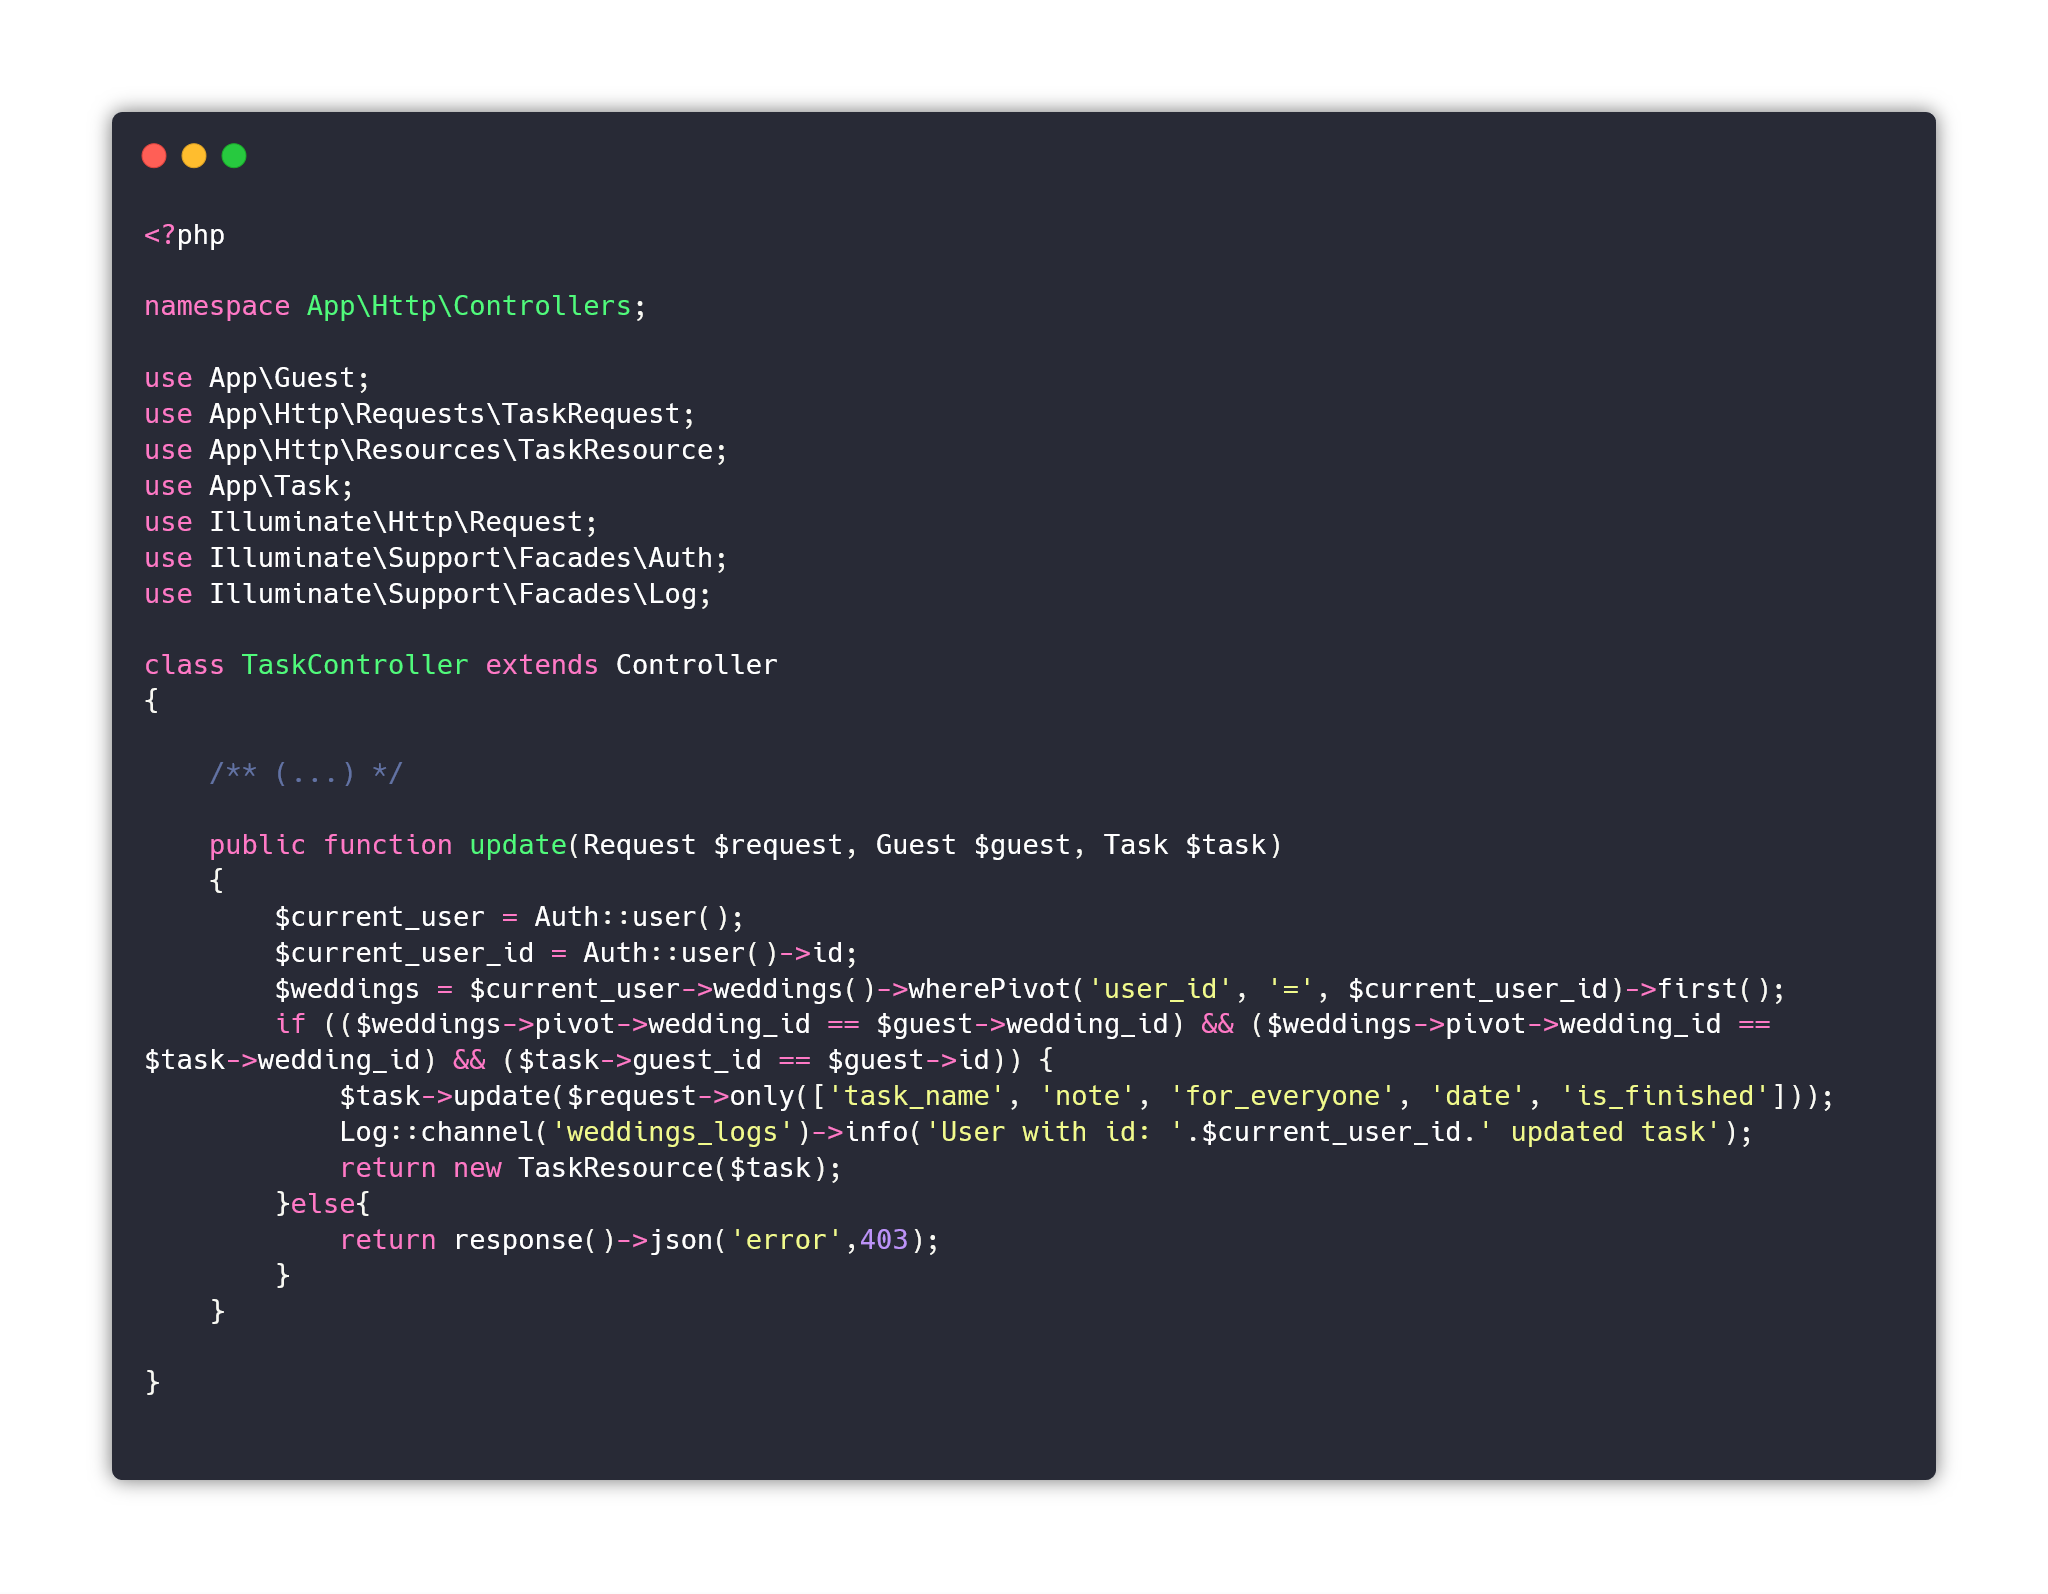
\includegraphics[width=\textwidth]{update.png}
		\footnotesize{(kod studentów, pisownia oryginalna)}
	\end{figure}
\end{frame}

\begin{frame}{Funkcje}
	Wcięcia i bloki bardzo ułatwiają czytanie funkcji. Ale ile poziomów wcięć jesteśmy w stanie zaakceptować w naszym kodzie?
\end{frame}

\begin{frame}
	\begin{figure} \centering
		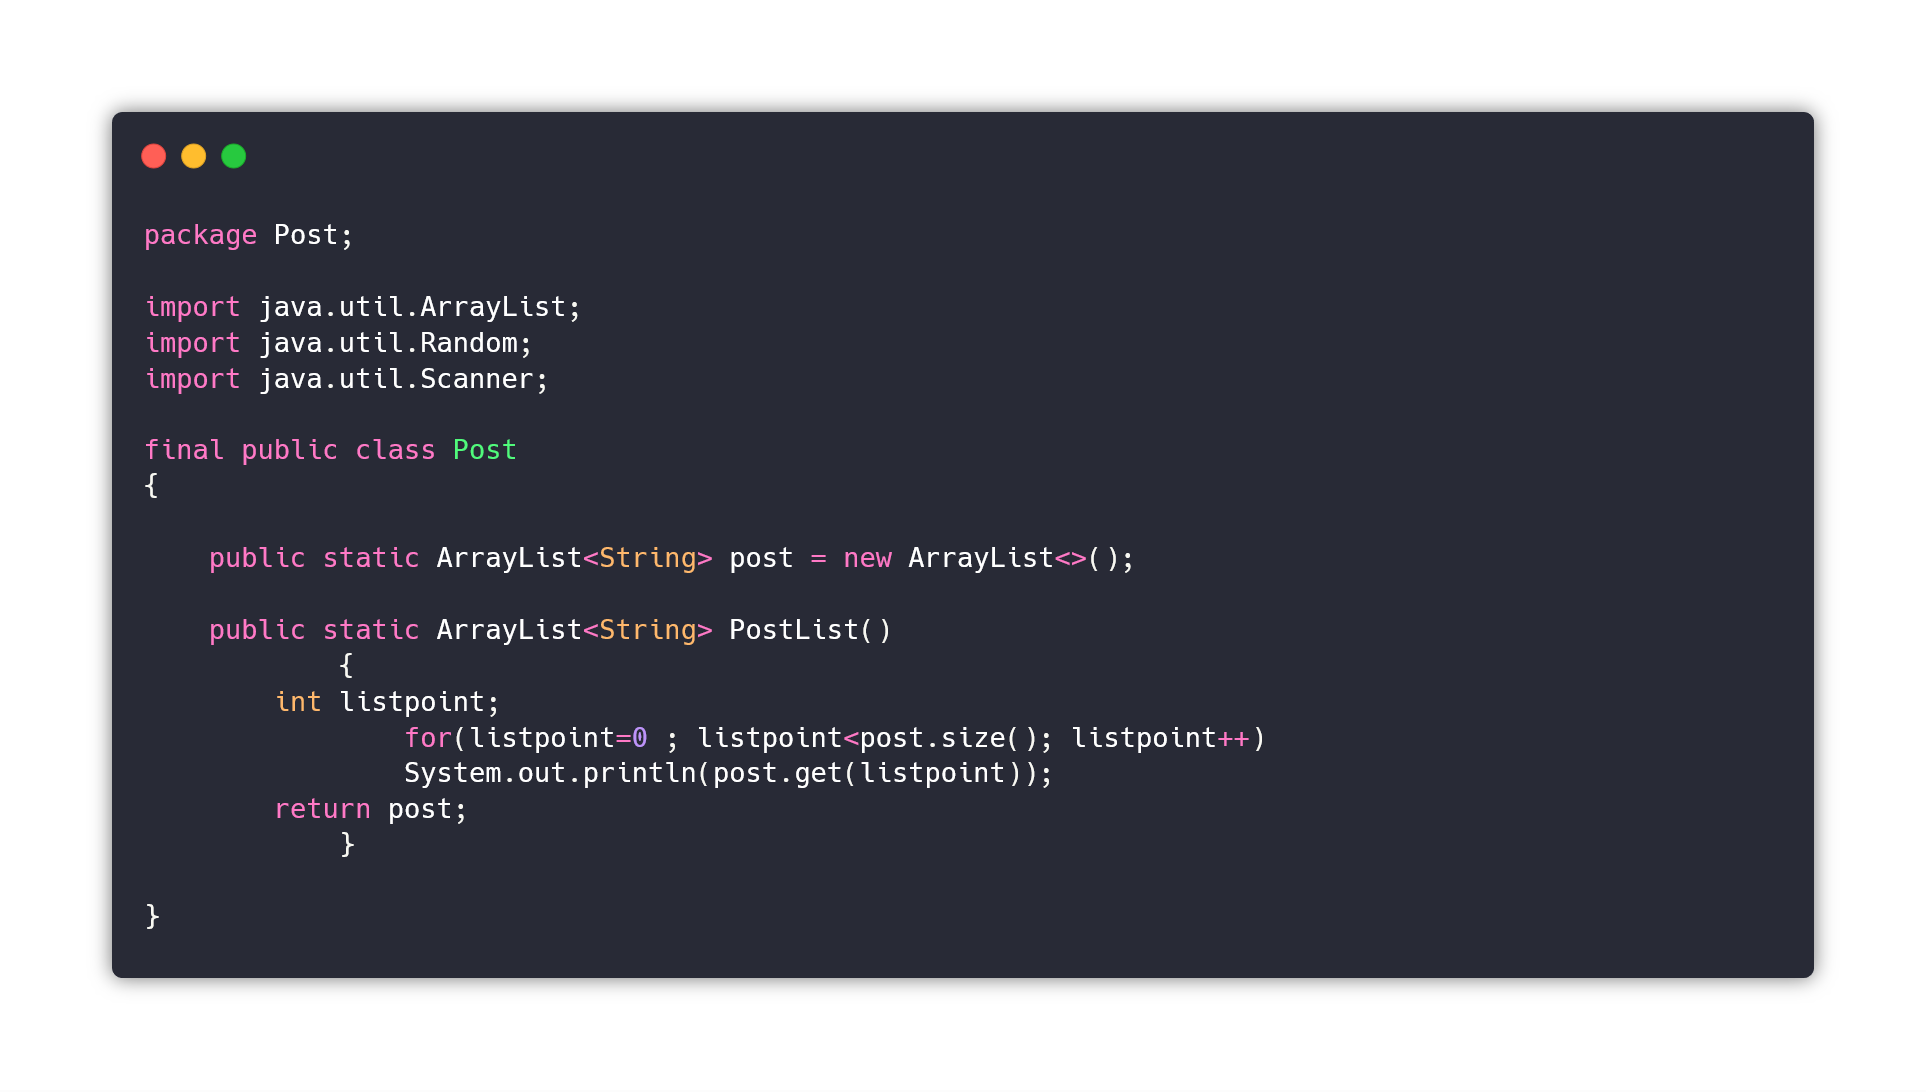
\includegraphics[width=\textwidth]{format.png}
		\footnotesize{(kod studentów, pisownia oryginalna)}
	\end{figure}
\end{frame}

\begin{frame}{Funkcje}
	I wracając jeszcze do SRP:
	
	\emph{Funkcje powinny wykonywać jedną operację.}
	
	\emph{Powinny to robić dobrze.}
	
	\emph{Powinny robić tylko to.}
\end{frame}

\begin{frame}
	\begin{figure} \centering
		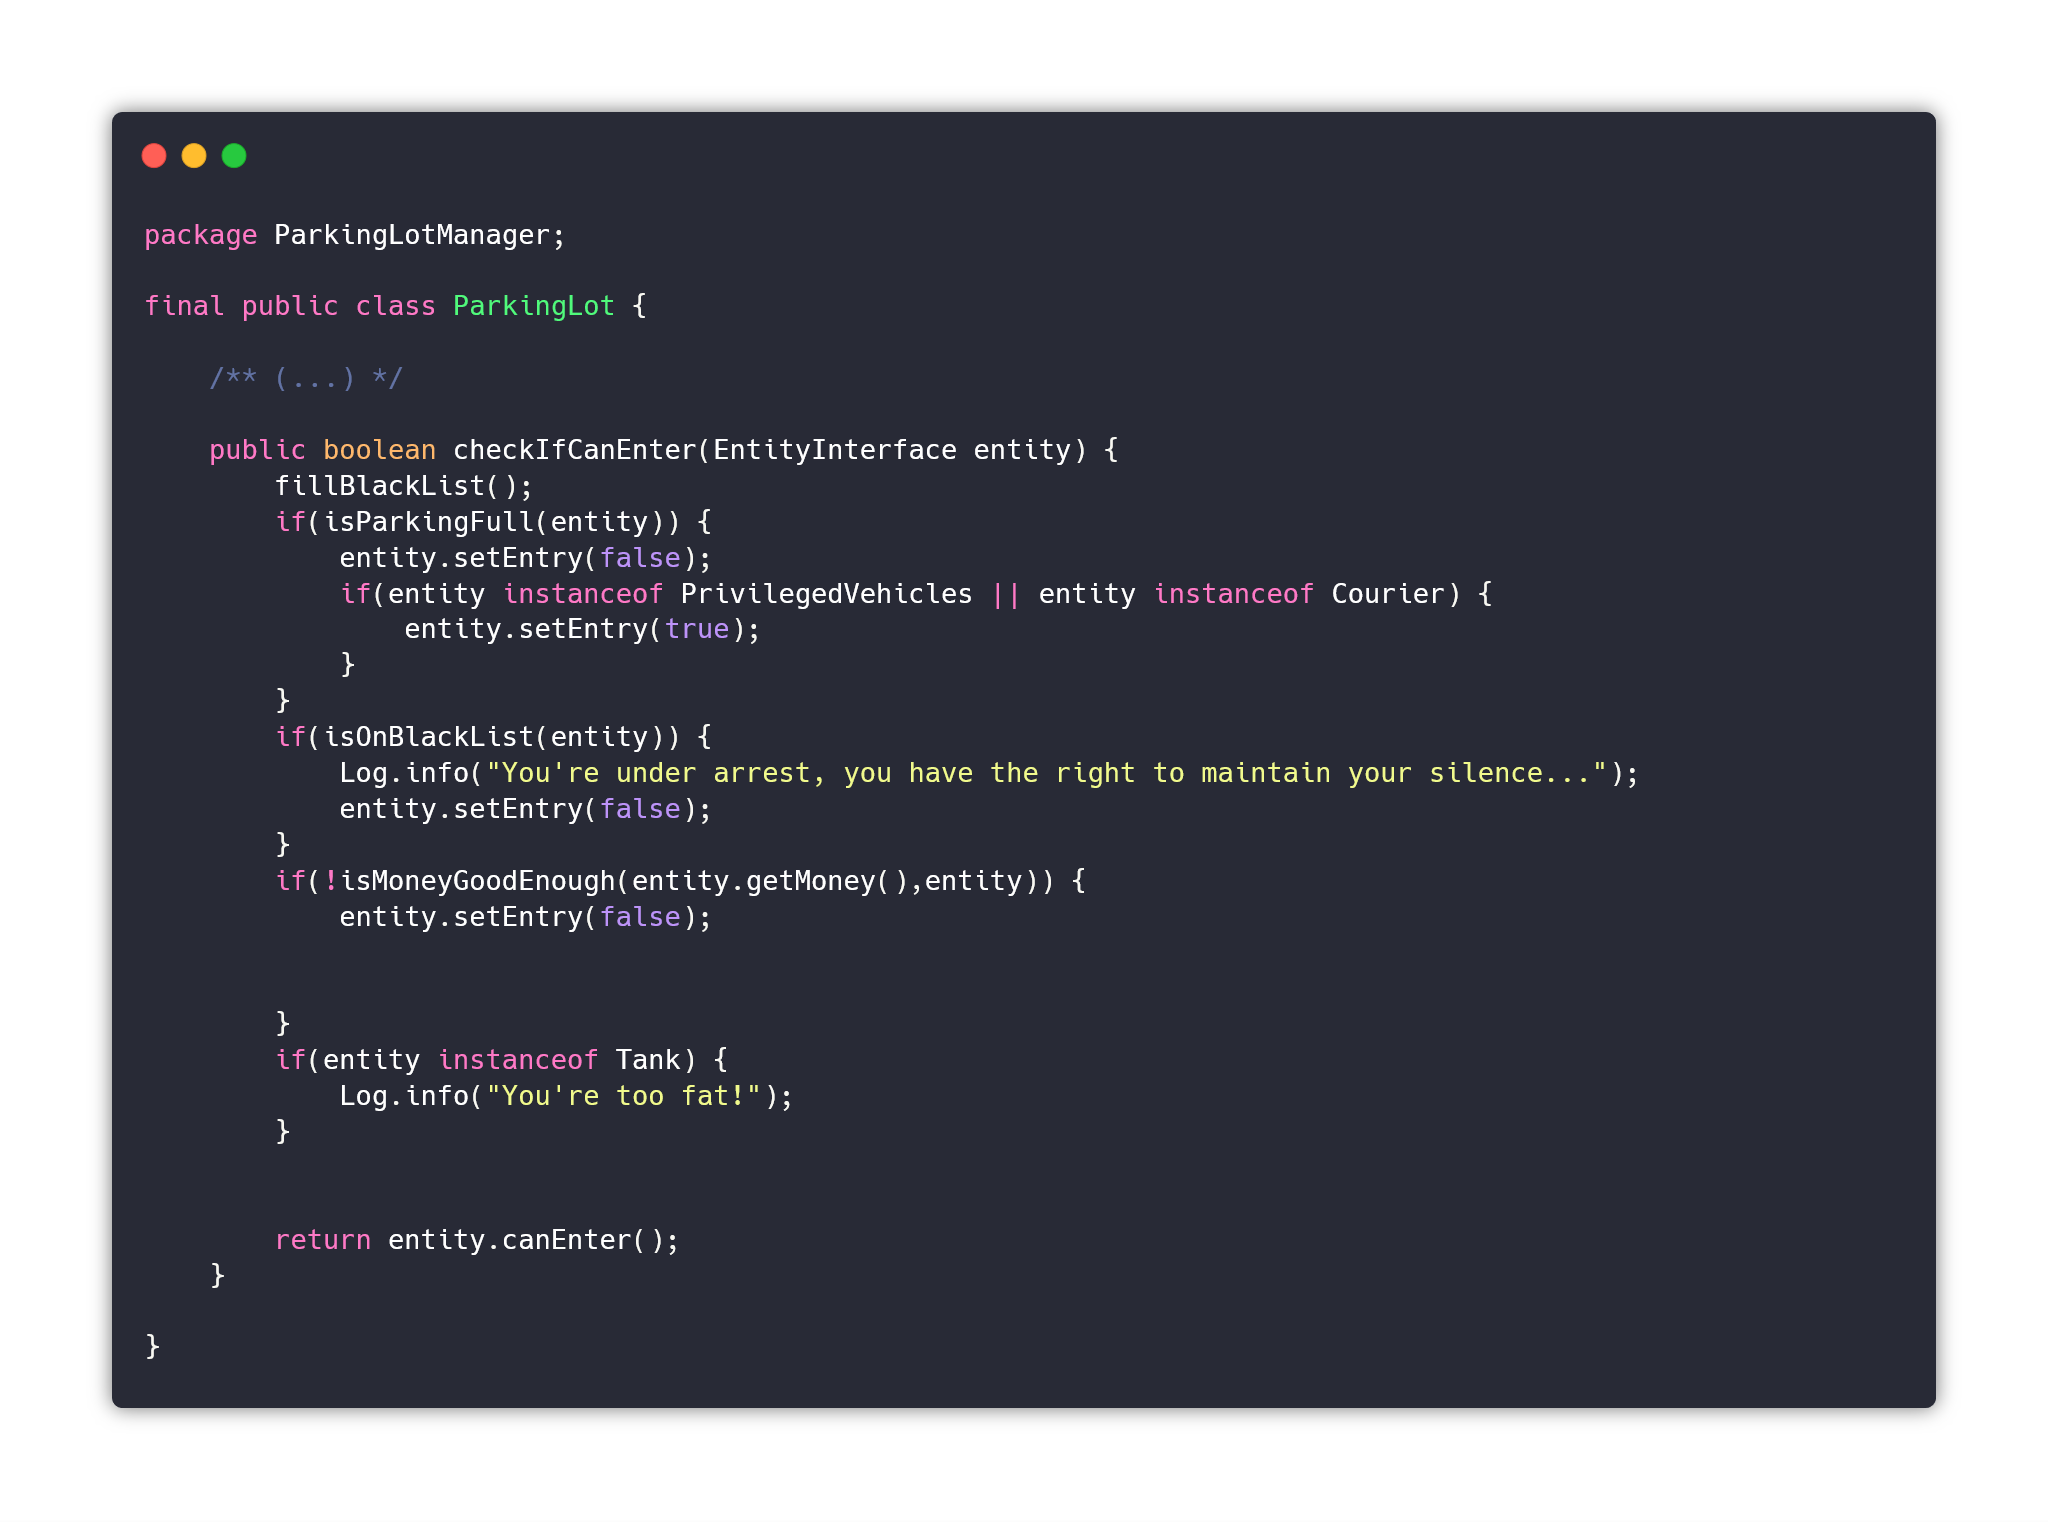
\includegraphics[width=\textwidth]{blahblah.png}
		\footnotesize{(kod studentów, pisownia oryginalna)}
	\end{figure}
\end{frame}

\begin{frame}{Funkcje}
	Skomplikowane \emph{switch-casy} czy zestawy \emph{ifów} bardzo zagrażają podstawowym zasadom tworzenia dobrego kodu. Czy istnieje sposób \emph{ulepszenia} poniższego kodu?
\end{frame}

\begin{frame}
	\begin{figure} \centering
		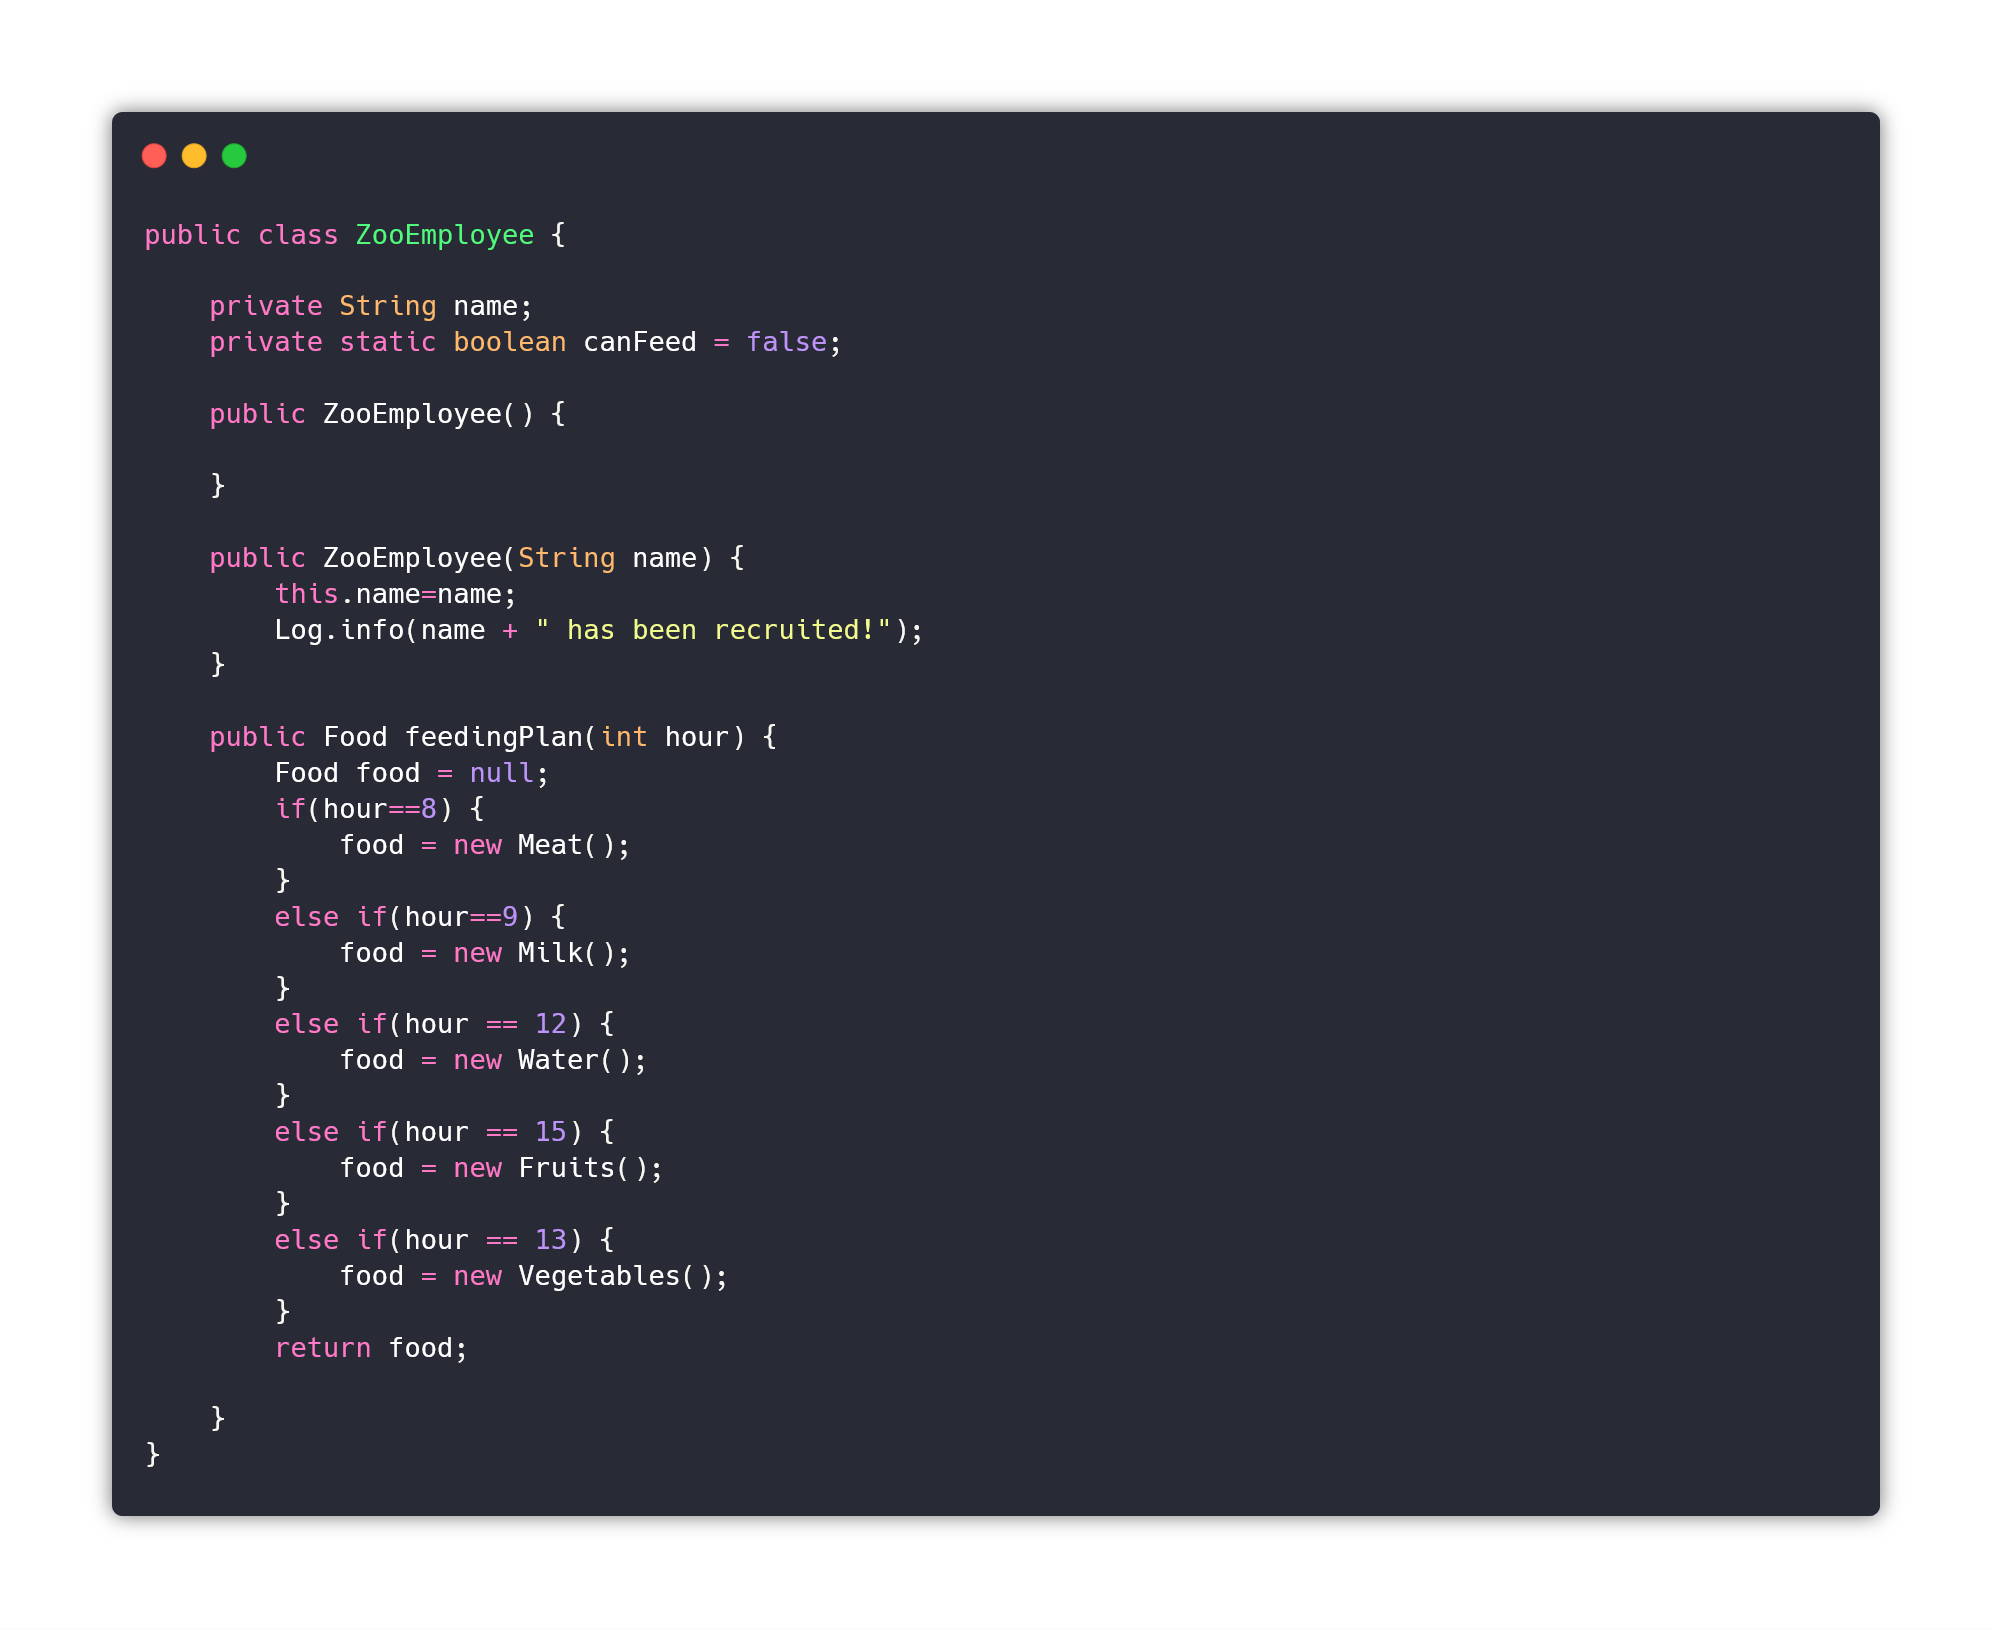
\includegraphics[width=\textwidth]{zoo.png}
		\footnotesize{(kod studentów, pisownia oryginalna)}
	\end{figure}
\end{frame}

\begin{frame}{Funkcje}
	\emph{Idealną liczbą argumentów dla funkcji jest zero (funkcja bezargumentowa). Następnie mamy jeden (jednoargumentowa) i dwa (dwuargumentowa).}
\end{frame}

\begin{frame}
	\begin{figure} \centering
		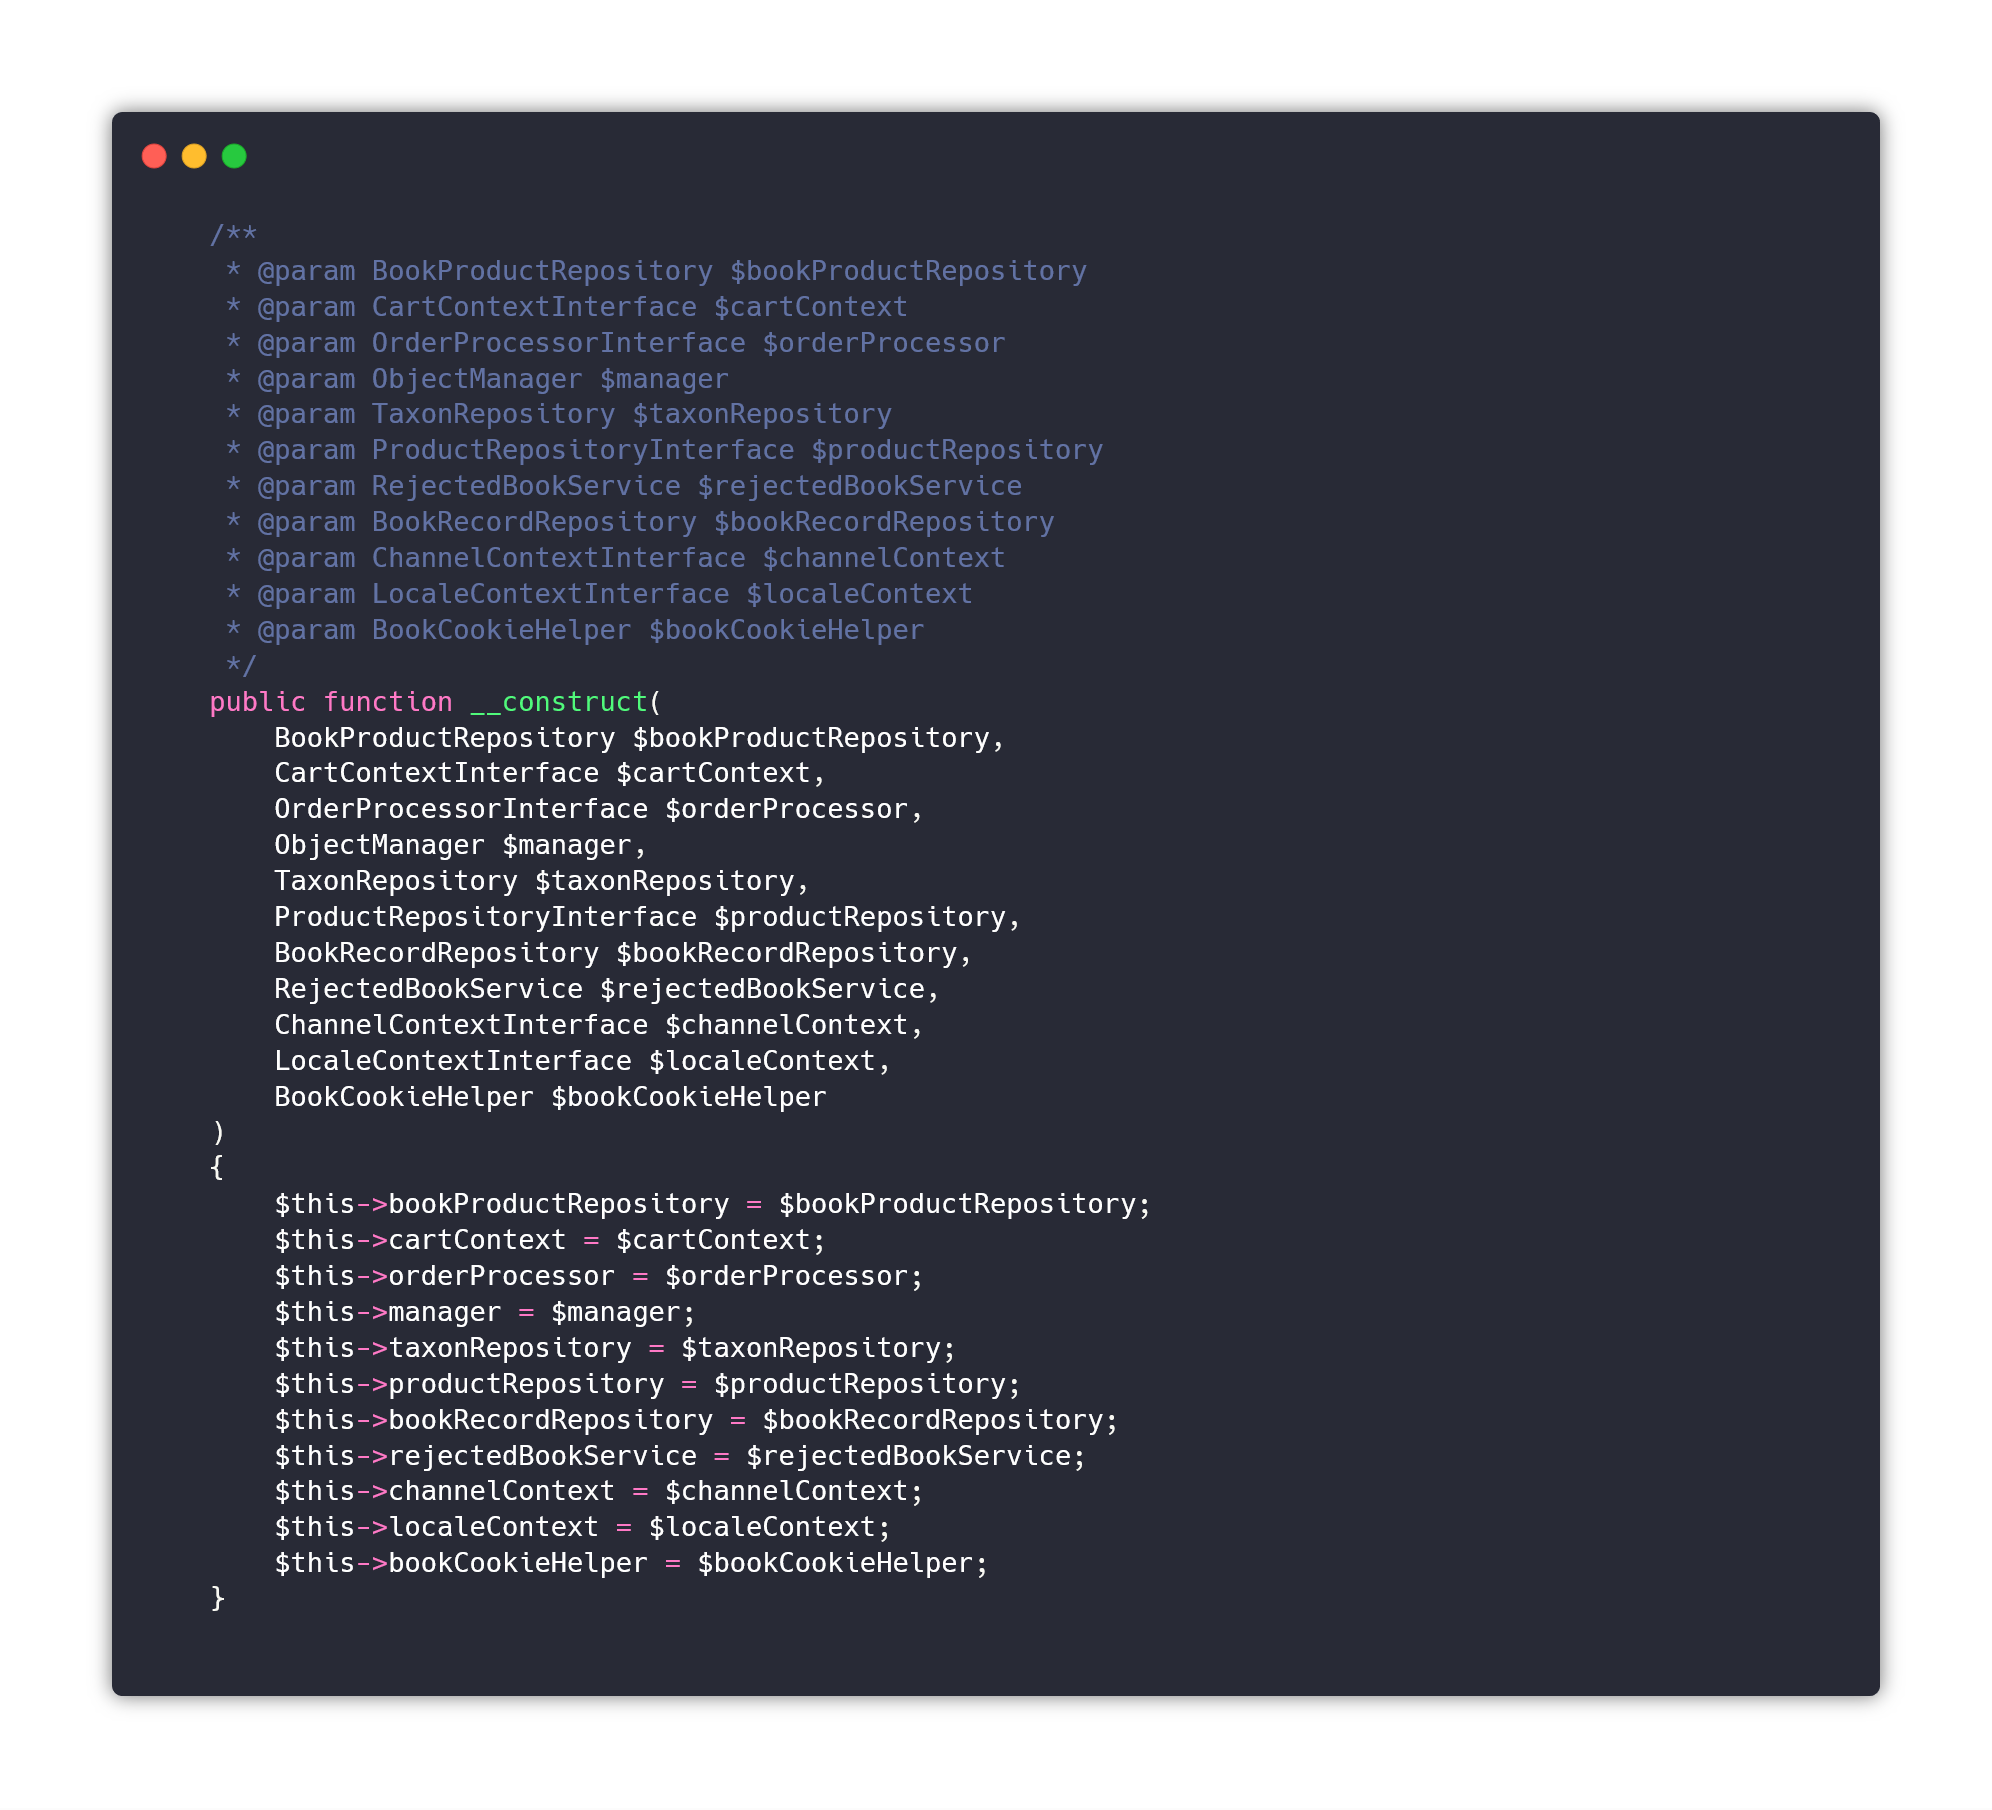
\includegraphics[width=\textwidth]{construct.png}
	\end{figure}
\end{frame}

\begin{frame}{Funkcje}
	Czy \emph{setter} powinien zwracać wynik? A może warto zastanowić się nad separacją zapytań od poleceń?
\end{frame}

\begin{frame}
	\begin{figure} \centering
		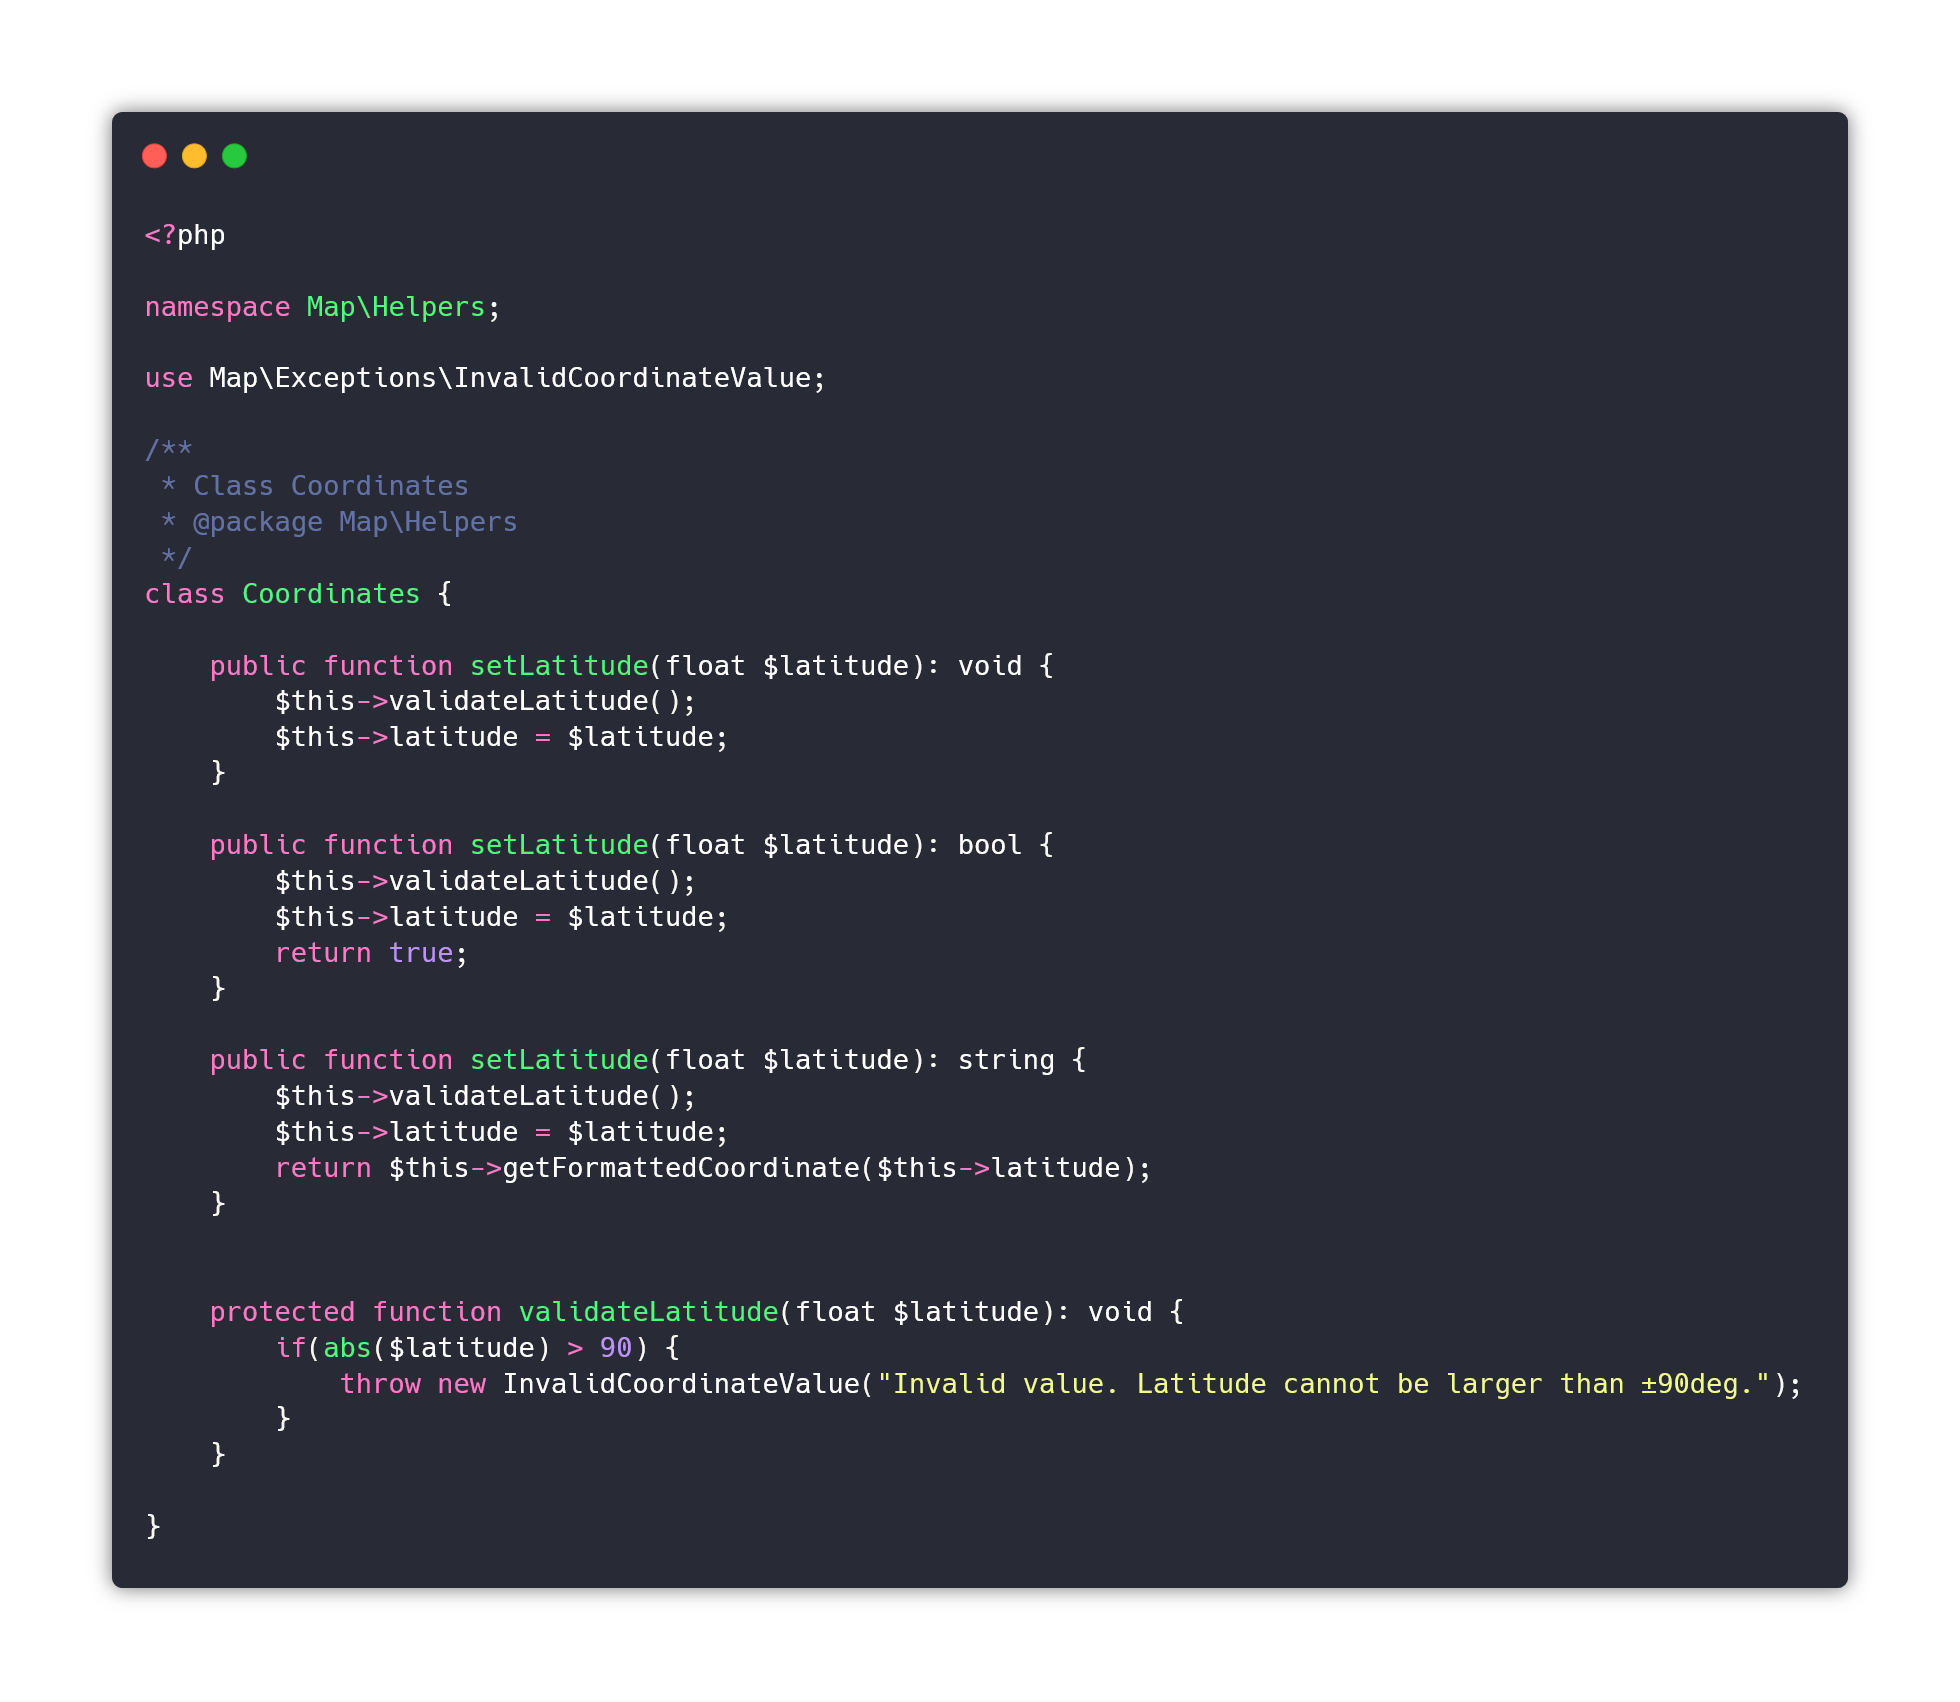
\includegraphics[width=\textwidth]{latitude.png}
	\end{figure}
\end{frame}

\begin{frame}{Funkcje}
	Jak powinny być obsługiwane błędy, których się spodziewamy? Czy funkcje powinny zwracać tylko to, czego oczekujemy? Jeżeli tak to w jakim formacie?
\end{frame}

\begin{frame}
	\begin{figure} \centering
		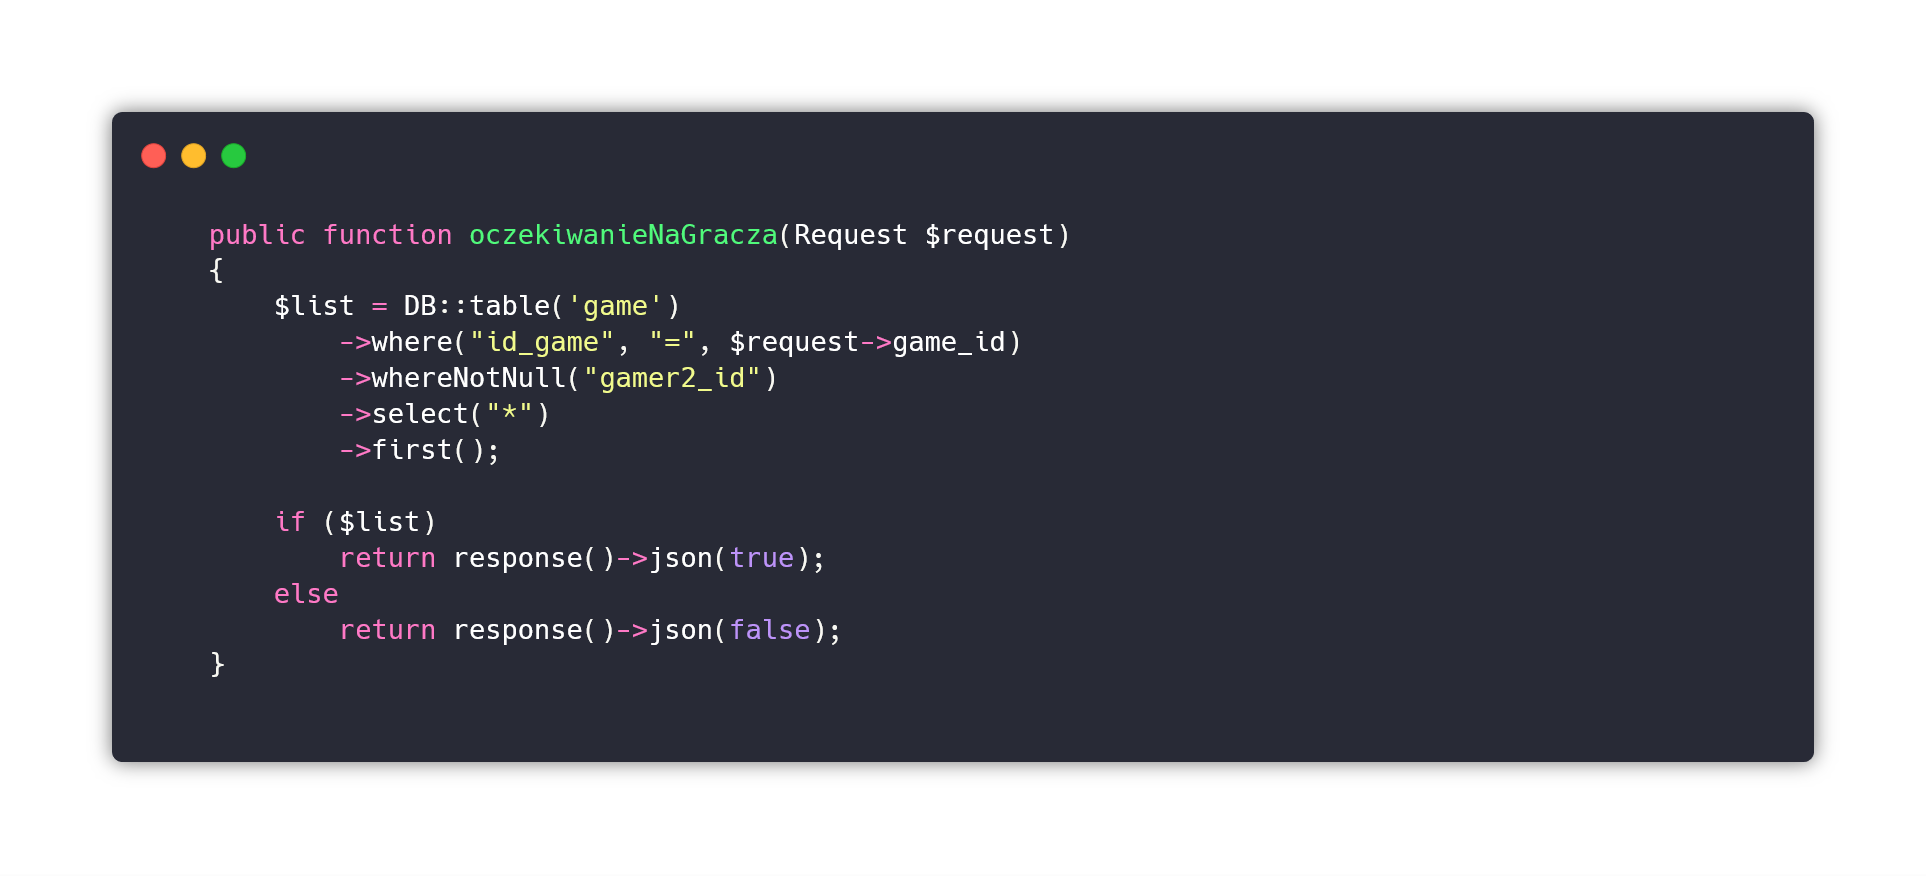
\includegraphics[width=\textwidth]{returny.png}
		\footnotesize{(kod studentów, pisownia oryginalna)}
	\end{figure}
\end{frame}

\begin{frame}{Funkcje}
	Kod poniżej pochodzi z zeszłosemestralnego studenckiego projektu. Co można byłoby w nim poprawić?
	
	\url{https://pastebin.com/raw/a0B72eik}
\end{frame}

\section{Formatowanie kodu}

\begin{frame}{Formatowanie}
	\emph{Formatowanie kodu jest ważne.}
	
	\emph{Jest zbyt ważne, aby je ignorować, i zbyt ważne, aby traktować je dogmatycznie. Formatowanie kodu ma zapewnić komunikację, a dobra komunikacja jest pierwszą zasadą biznesu zawodowego programisty.}
\end{frame}

\begin{frame}{Formatowanie}
	Warto wykorzystać pojęcie \emph{gęstości pionowej} i zewrzeć ze sobą wiersze mające ścisłe związki ze sobą.
\end{frame}

\begin{frame}
	\begin{figure} \centering
		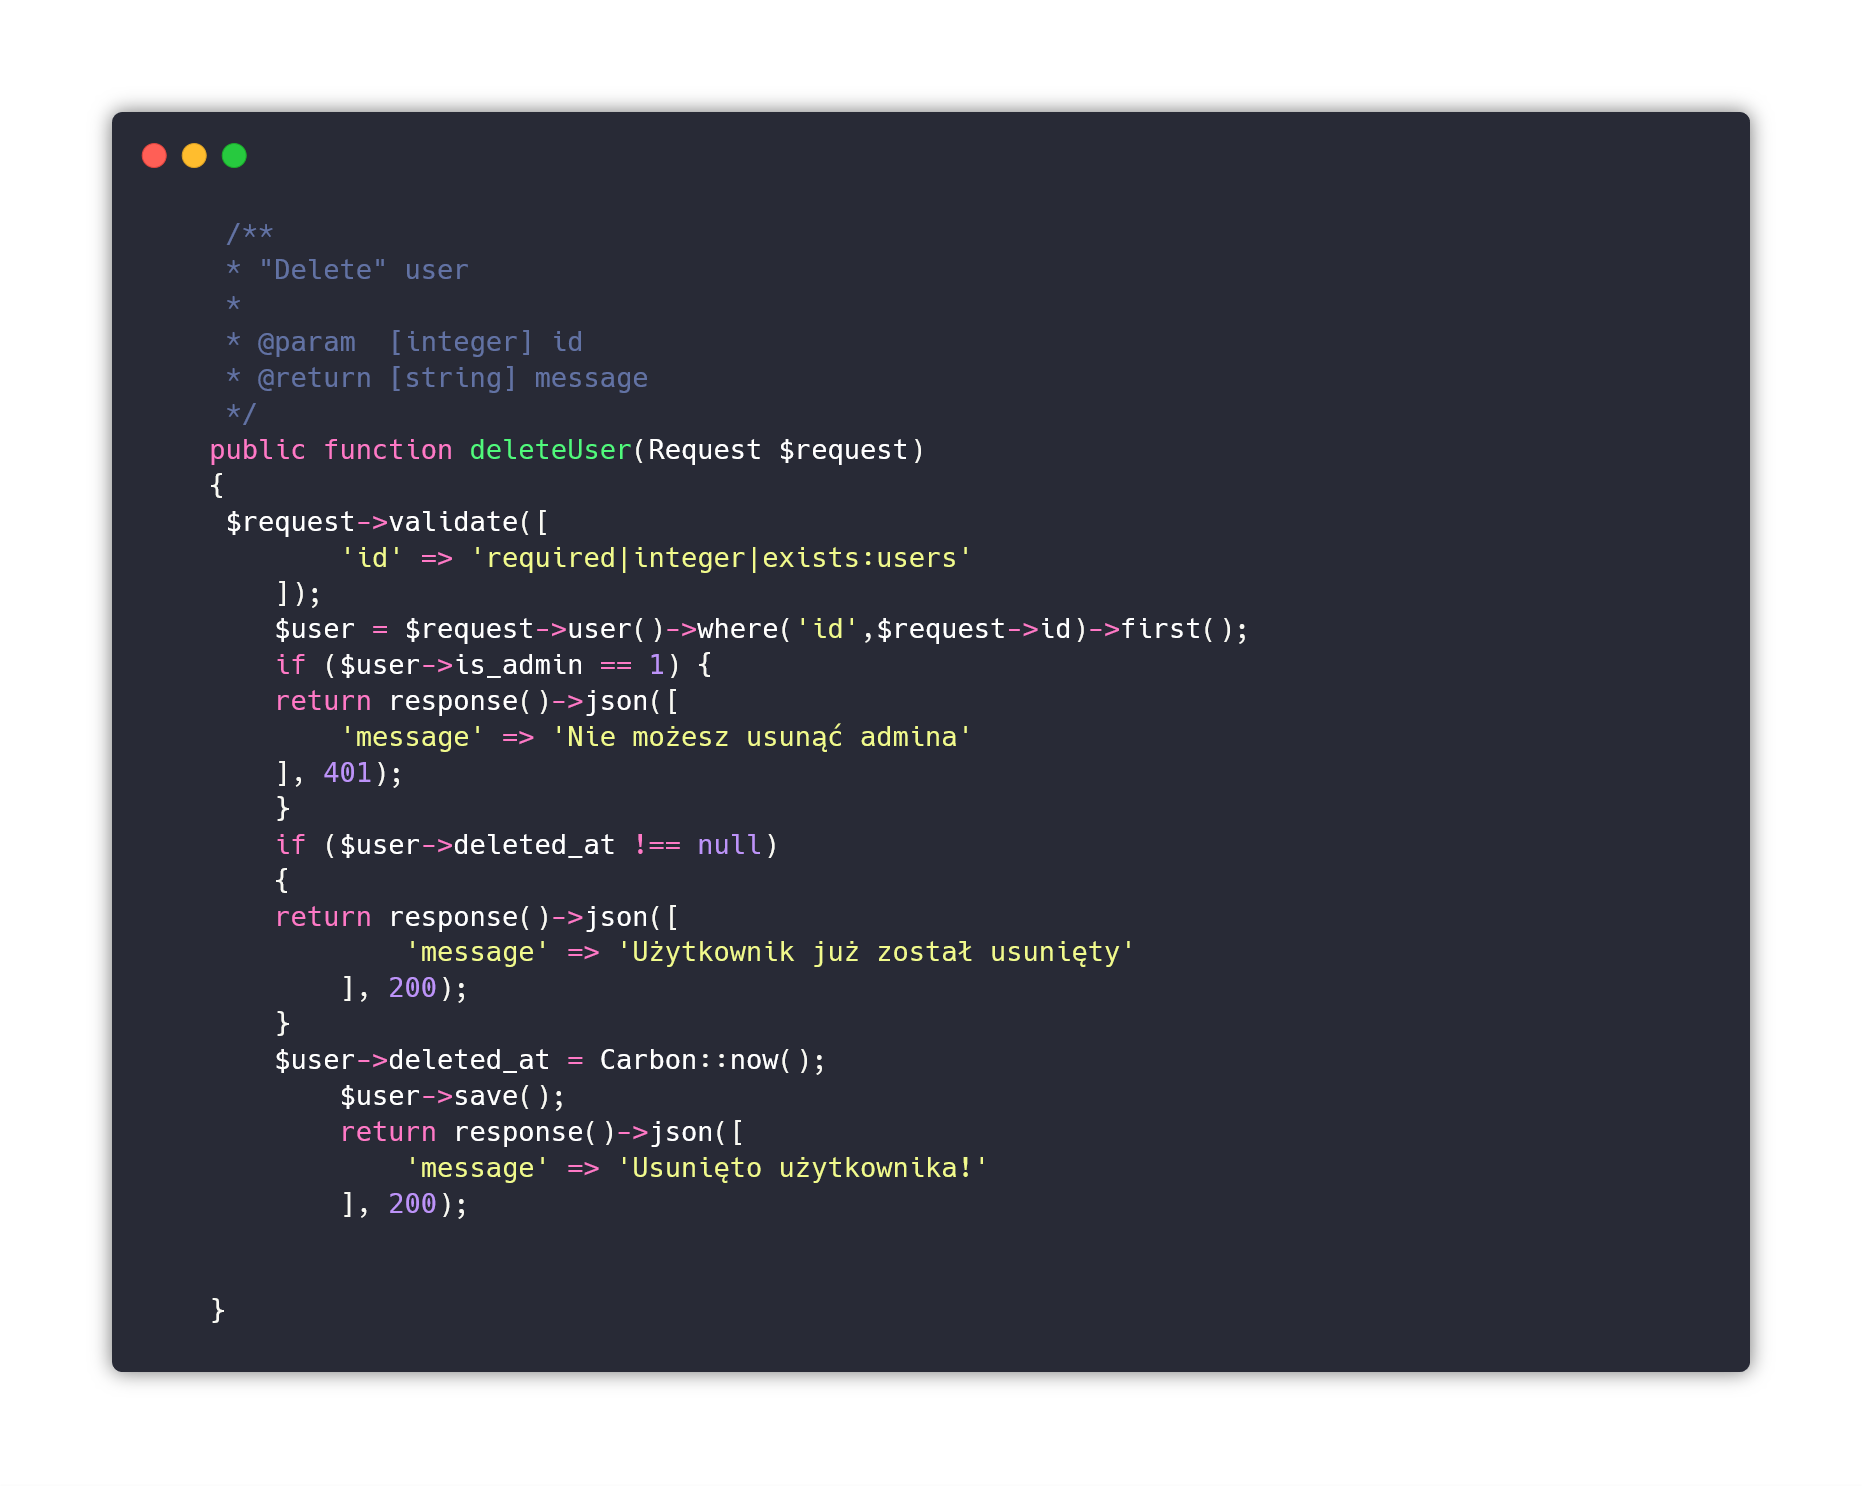
\includegraphics[width=\textwidth]{oh.png}
		\footnotesize{(kod studentów, pisownia oryginalna)}
	\end{figure}
\end{frame}

\begin{frame}
	\begin{figure} \centering
		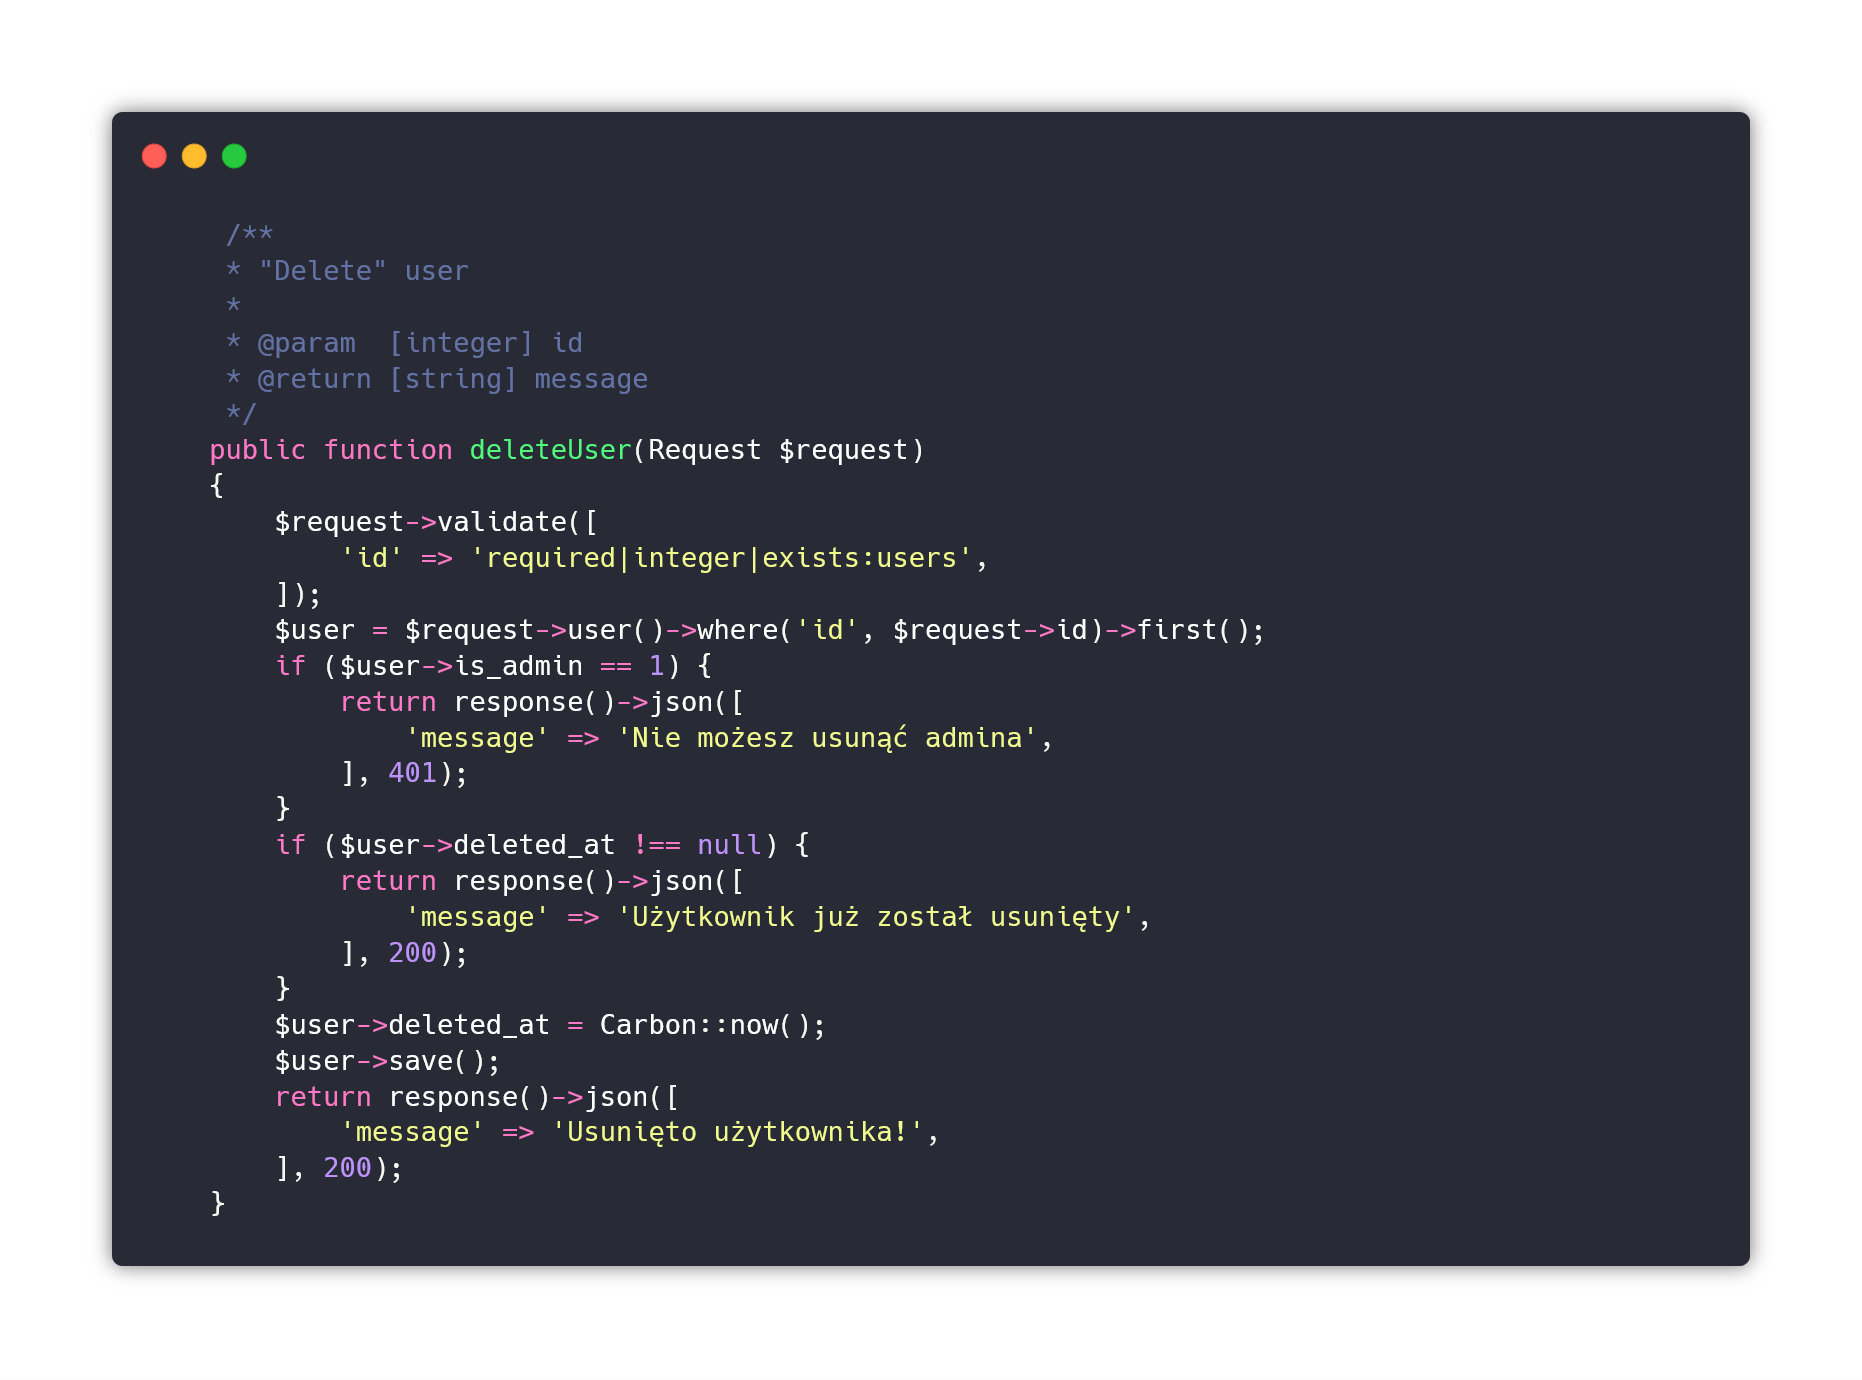
\includegraphics[width=\textwidth]{oh2.png}
		\footnotesize{(kod studentów, po autoformacie)}
	\end{figure}
\end{frame}

\begin{frame}
	\begin{figure} \centering
		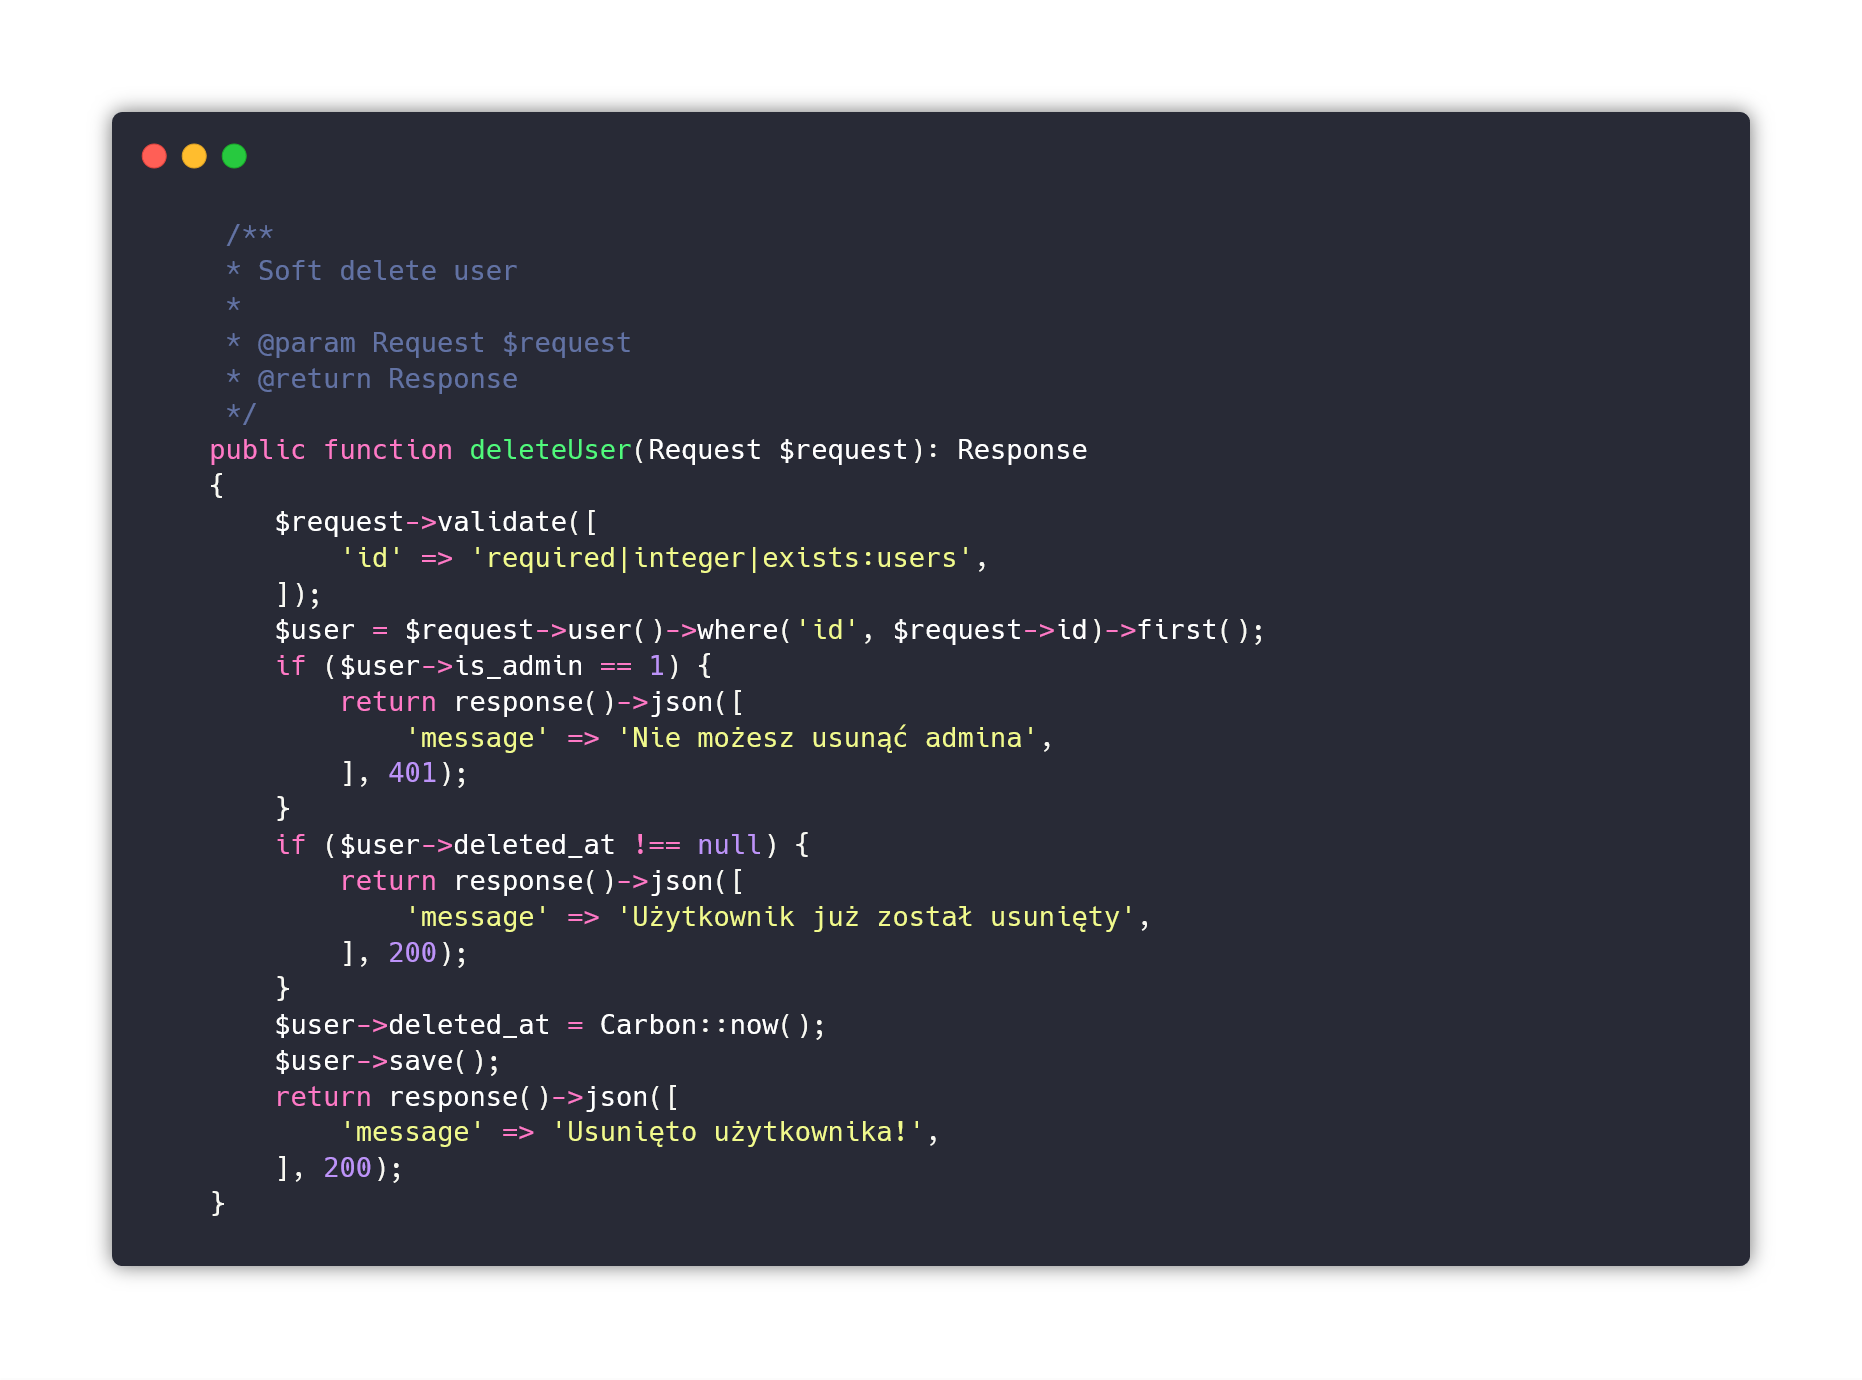
\includegraphics[width=\textwidth]{oh3.png}
		\footnotesize{(kod studentów, po zmianie opisu funkcji)}
	\end{figure}
\end{frame}

\begin{frame}
	\begin{figure} \centering
		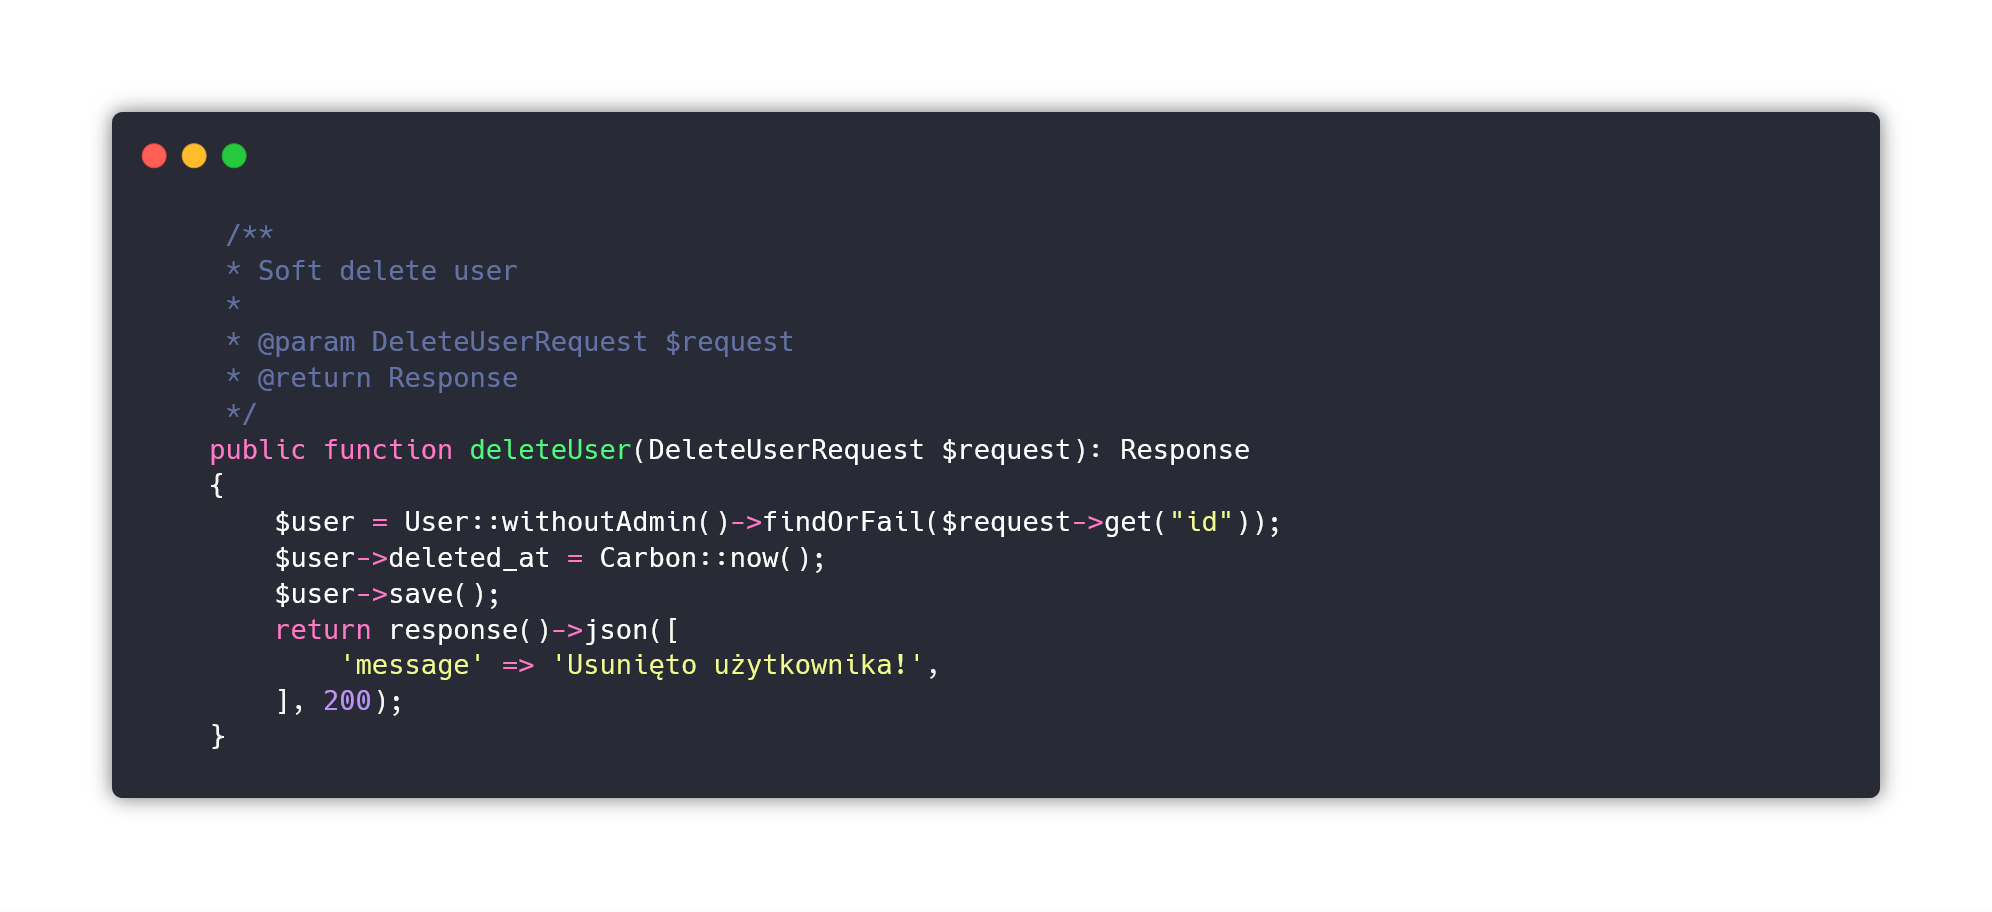
\includegraphics[width=\textwidth]{oh4.png}
		\footnotesize{(kod studentów, po oczyszczeniu funkcji)}
	\end{figure}
\end{frame}

\begin{frame}
	\begin{figure} \centering
		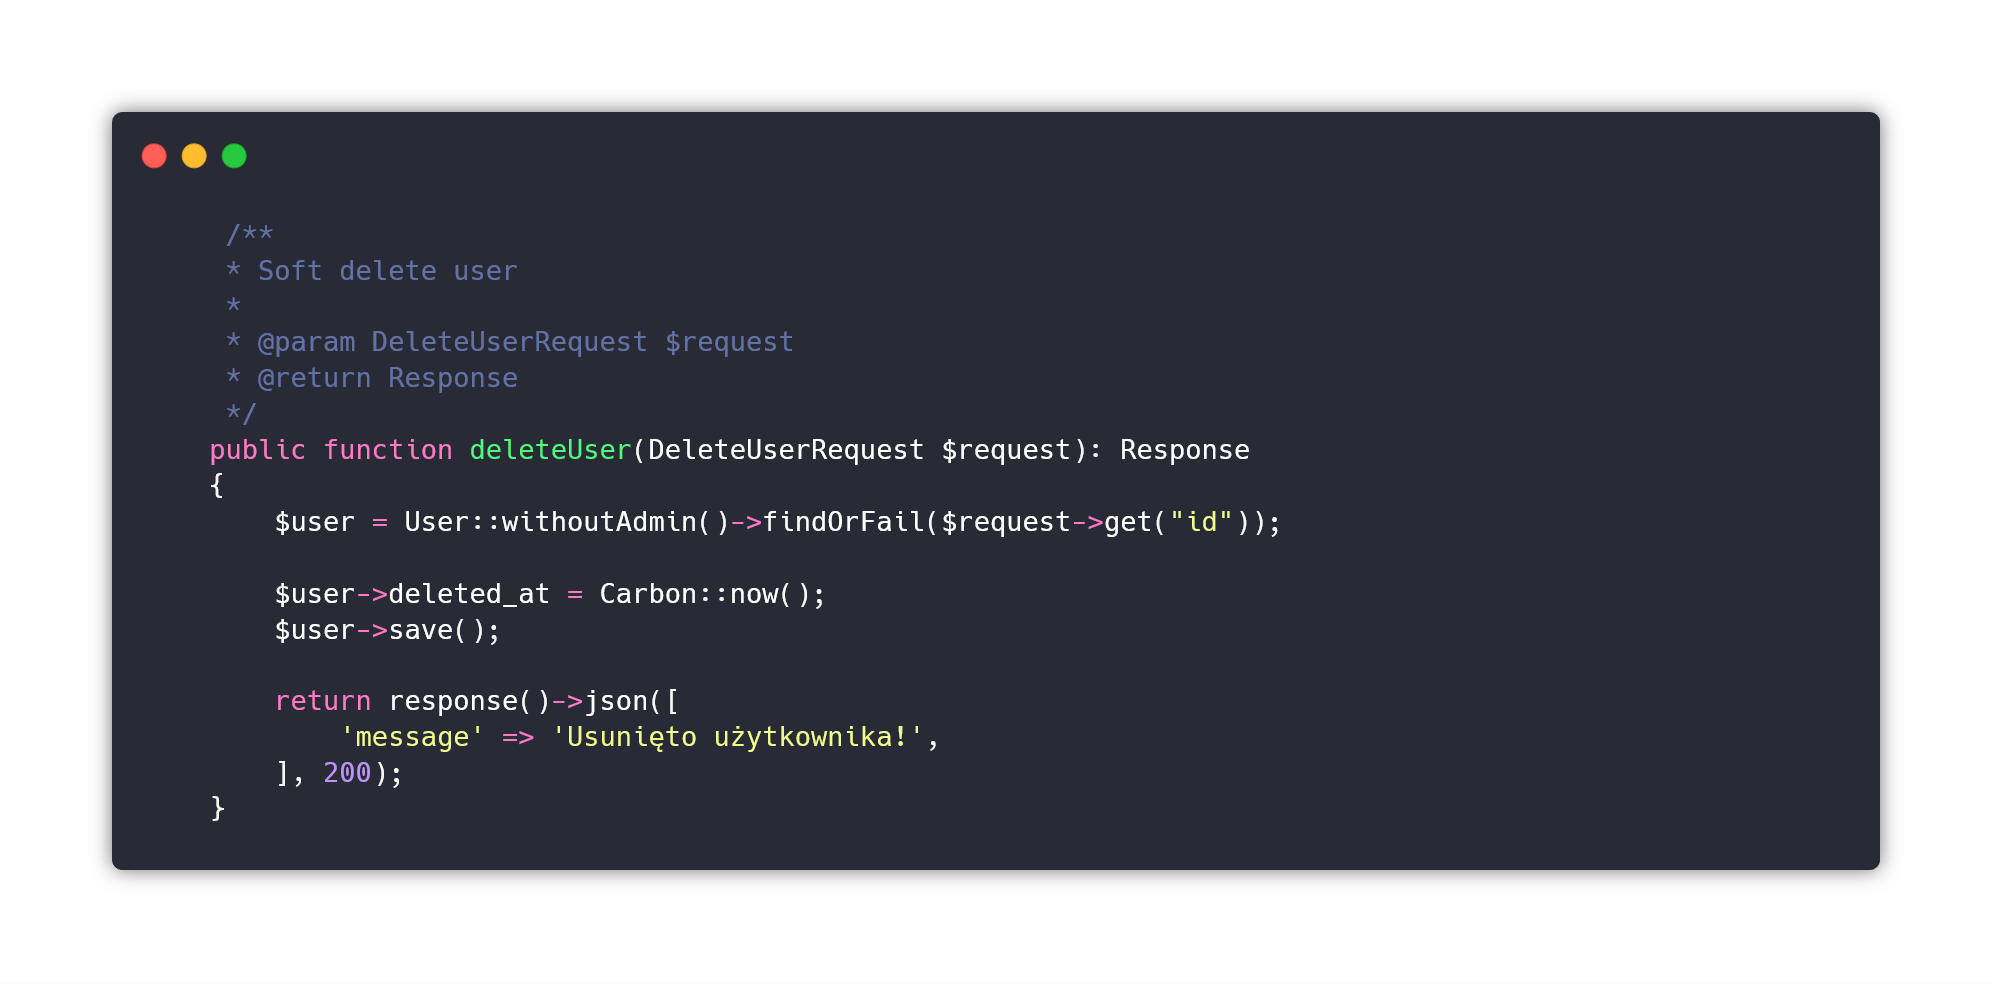
\includegraphics[width=\textwidth]{oh5.png}
		\footnotesize{(kod studentów, po zwiększeniu pionowych odstępów)}
	\end{figure}
\end{frame}

\begin{frame}{Formatowanie}
	Dobrym zwyczajem może być układanie metod w klasie pod względem ich znaczenia.
	
	\emph{Wywoływana funkcja powinna znajdować się poniżej funkcji wywołującej.}
\end{frame}

\begin{frame}
	\begin{figure} \centering
		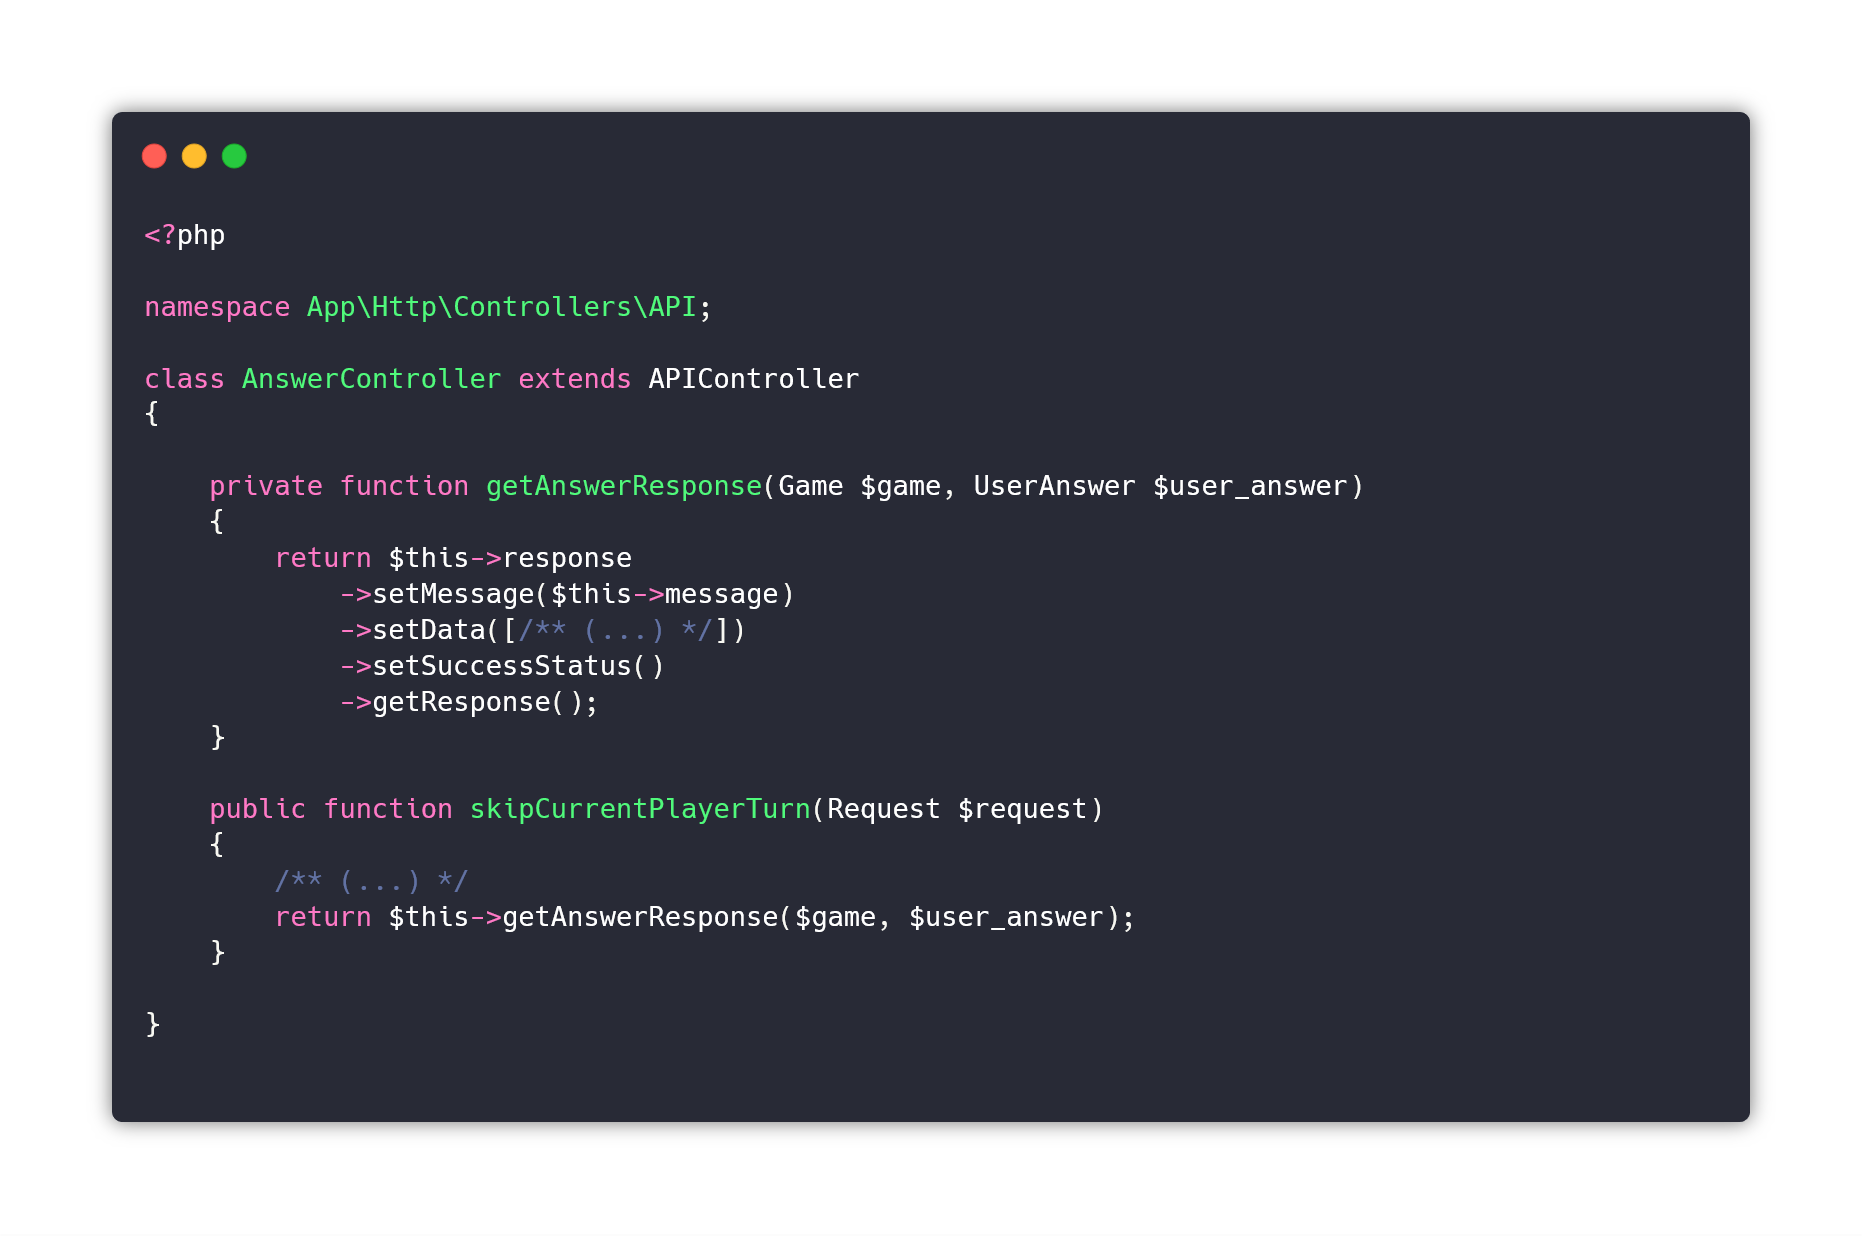
\includegraphics[width=\textwidth]{order.png}
		\footnotesize{(kod studentów, pisownia oryginalna)}
	\end{figure}
\end{frame}

\begin{frame}{Formatowanie}
	Wiersze nie powinny być zbyt długie, ale nigdy nie powinien być to kontrargument dla pisania kodu bez odstępów.
\end{frame}

\begin{frame}
	\begin{figure} \centering
		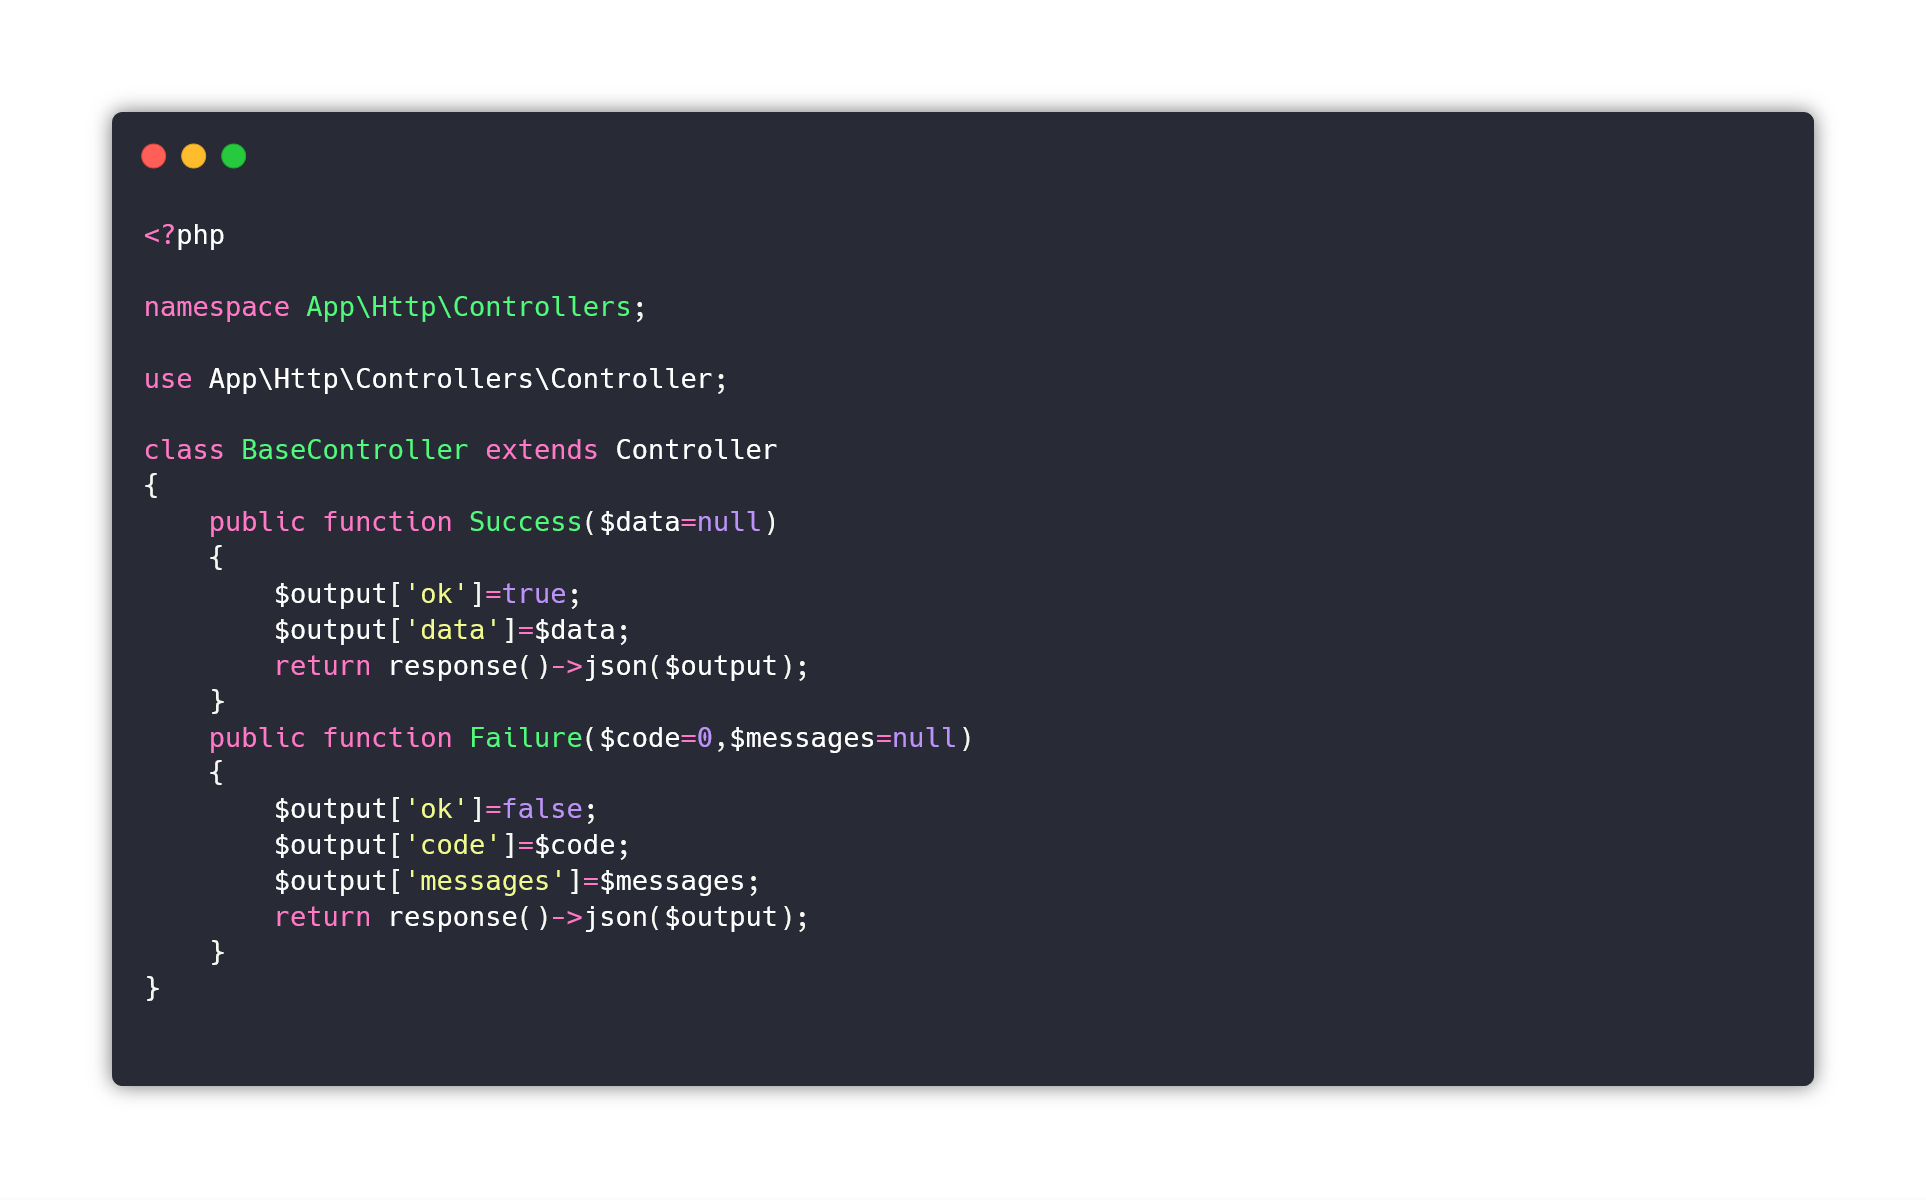
\includegraphics[width=\textwidth]{spaces.png}
		\footnotesize{(kod studentów, pisownia oryginalna)}
	\end{figure}
\end{frame}

\begin{frame}{Formatowanie}
	Nie warto przejmować się natomiast udziwnieniami formatowania kodu, które z różnych przyczyn są popularne w niektórych środowiskach. Najważniejsza jest czytelność.
\end{frame}

\begin{frame}
	\begin{figure} \centering
		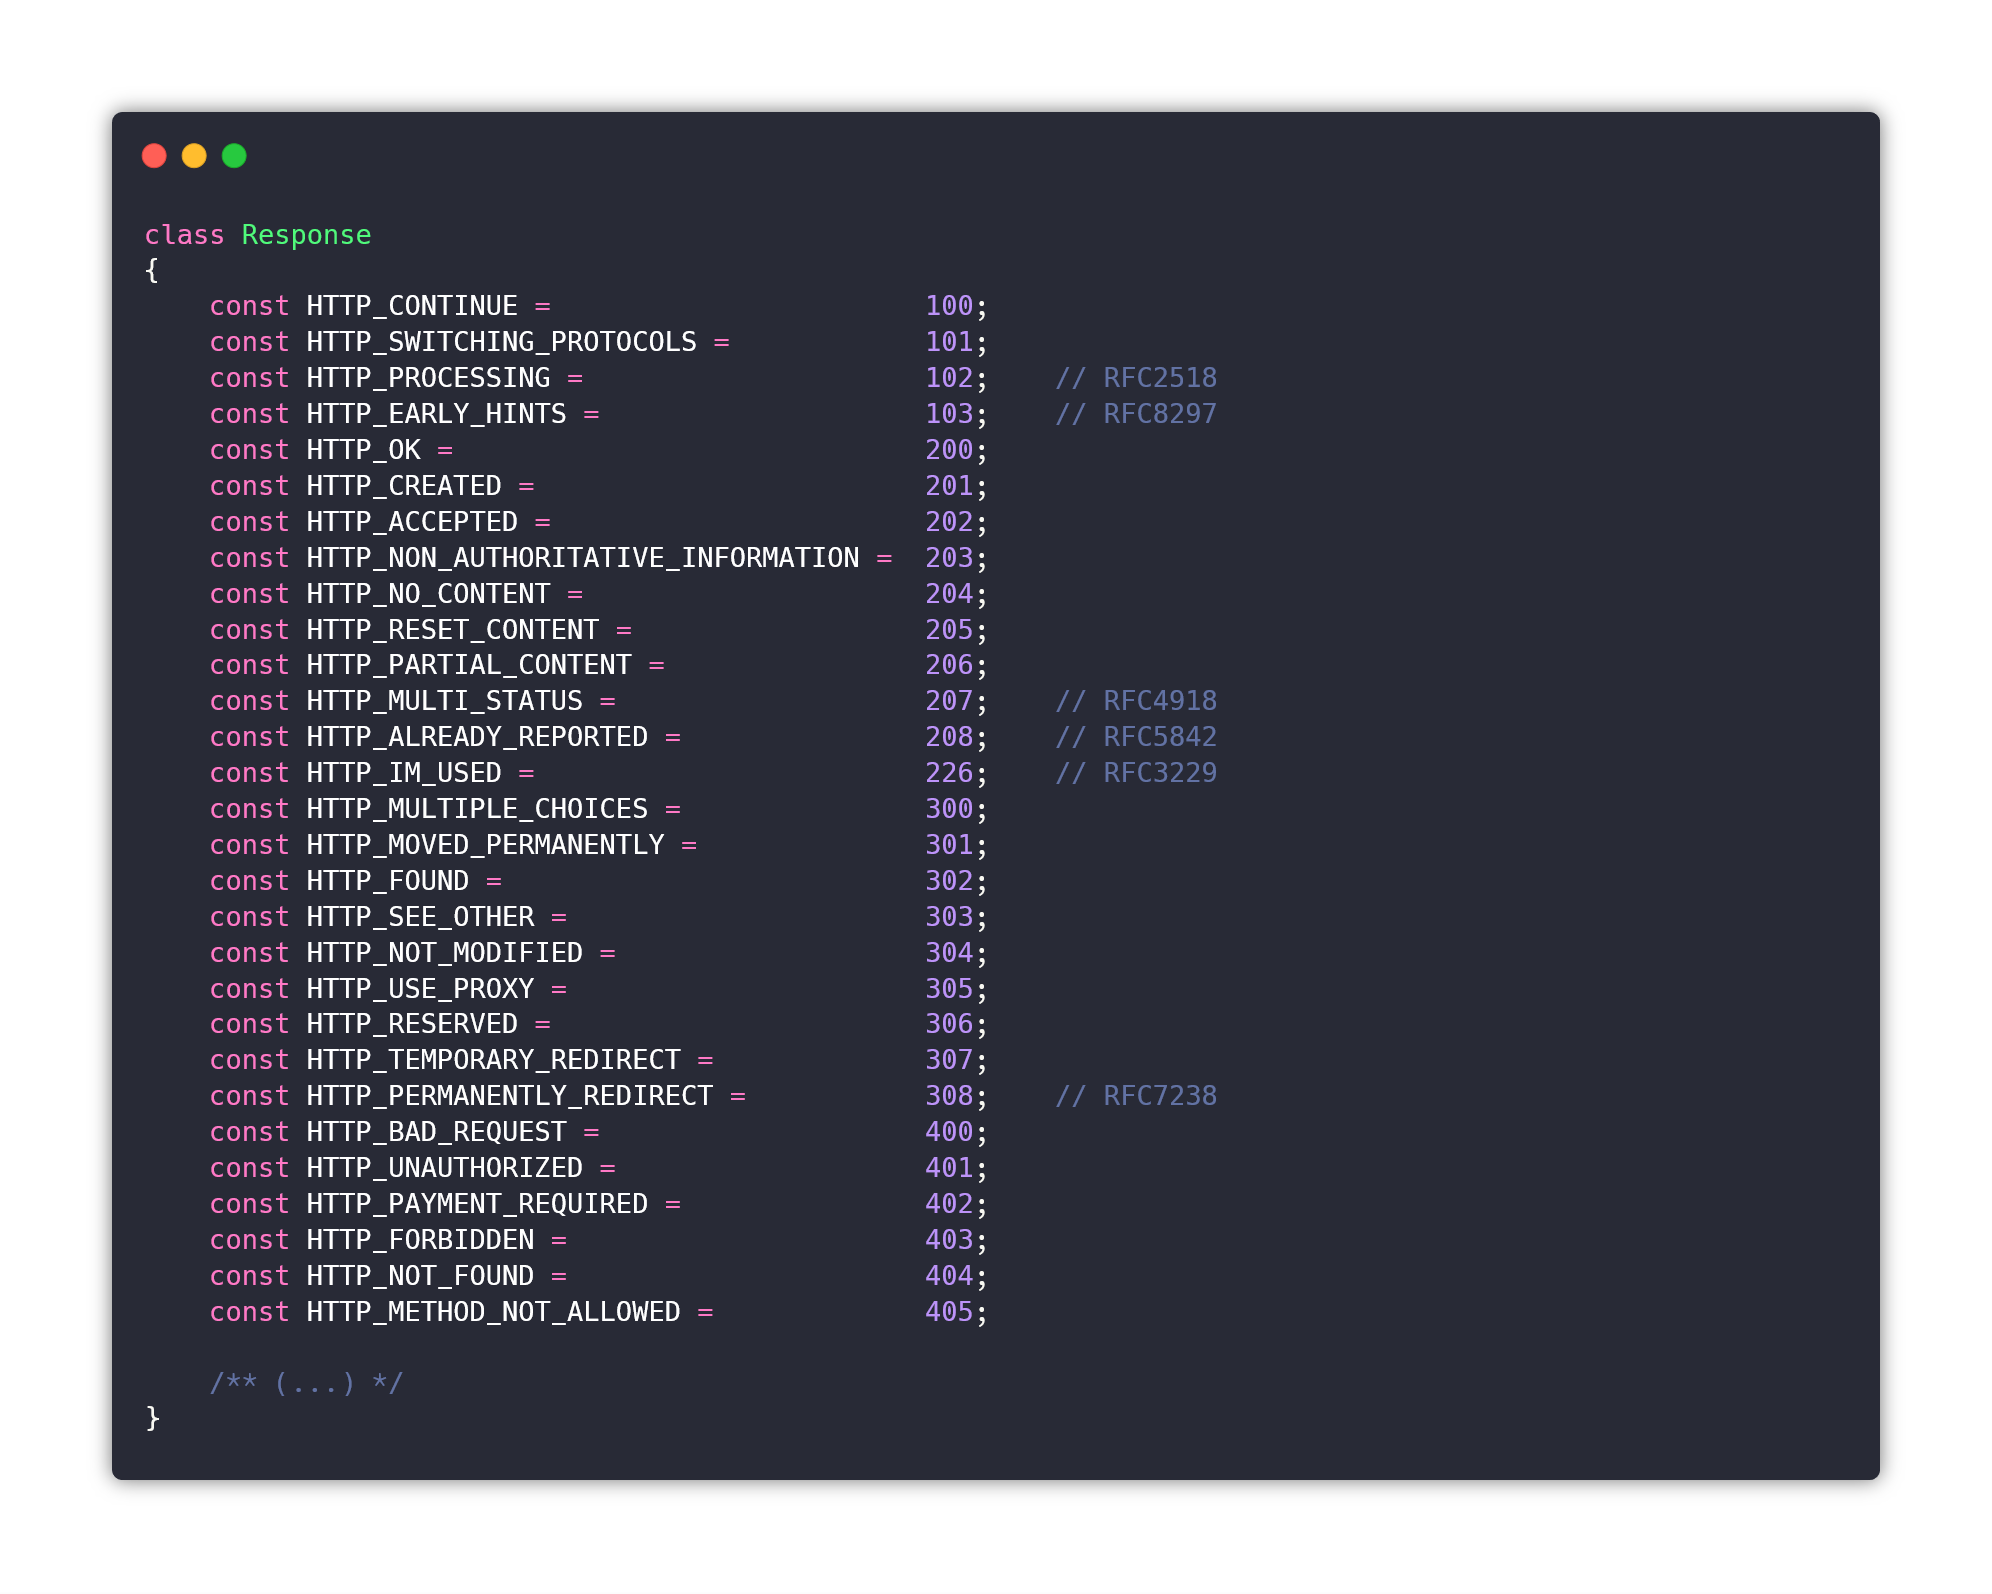
\includegraphics[width=\textwidth]{const.png}
	\end{figure}
\end{frame}

\begin{frame}{Formatowanie}
	Wcięcia to podstawa. 
	
	\emph{Nasze oko może szybko określić strukturę wcięć w pliku. Można niemal natychmiast odszukać zmienne, konstruktory, akcesory i metody.}
\end{frame}

\begin{frame}
	\begin{figure} \centering
		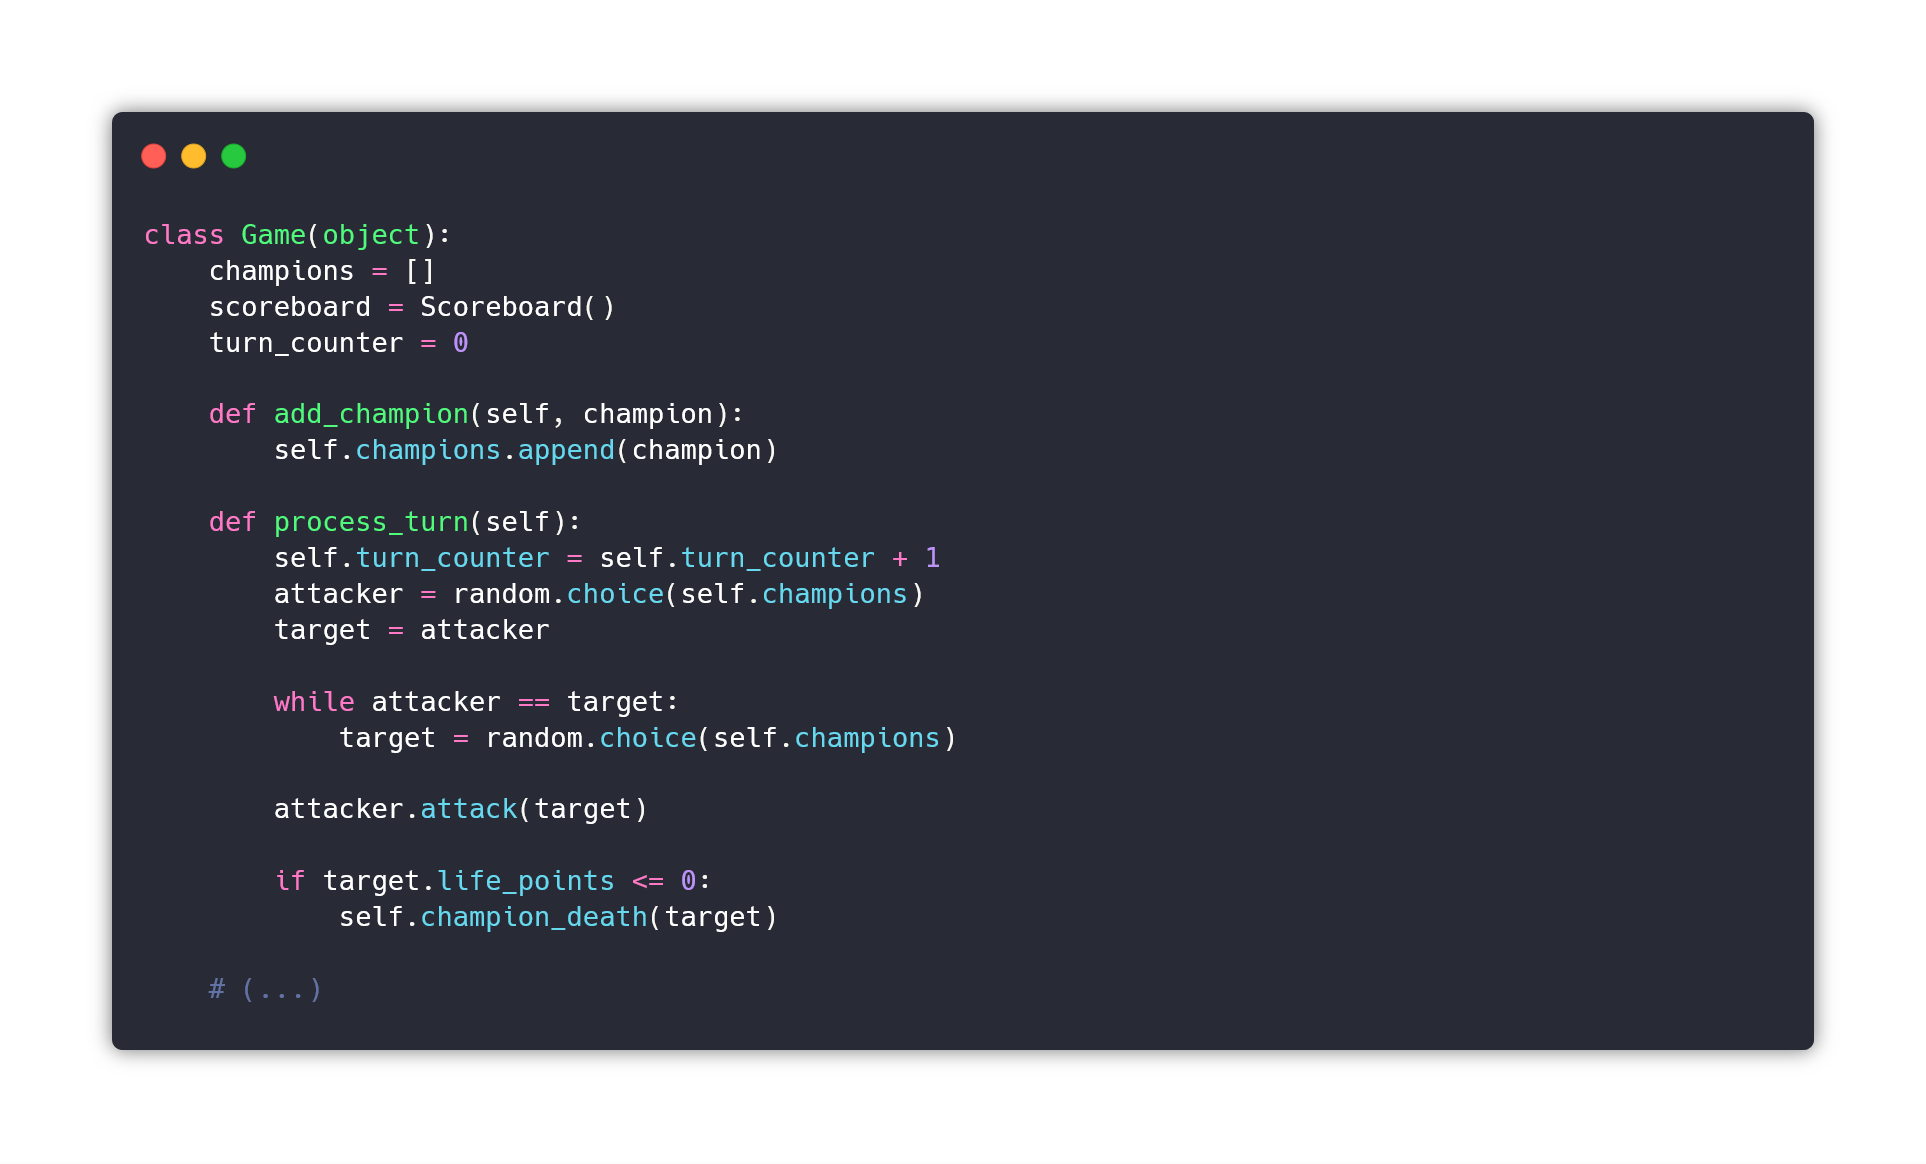
\includegraphics[width=\textwidth]{python.png}
		\footnotesize{(kod studentów, pisownia oryginalna)}
	\end{figure}
\end{frame}

\section{Podsumowanie}

\appendix

\begin{frame}[standout]
	Pytania?
\end{frame}

\begin{frame}{}

	Kod prezentacji dostępny jest w repozytorium git pod adresem \texttt{https://bitbucket.org/krewak/pwsz-ppsi} \\ \ \\

	\begin{figure}
		\centering
		\href{https://bitbucket.org/krewak/pwsz-ppsi}{
			
\includegraphics[width=.15\textwidth]{../_template/bitbucket.png}
		}
	\end{figure}
	
	Wszystkie informacje dot. kursu dostępne są pod adresem \texttt{http://pwsz.rewak.pl/kursy/4} \\ \ \\

	\begin{figure}
		\centering
		\href{http://pwsz.rewak.pl/kursy/3}{
			
\includegraphics[width=.15\textwidth]{../_template/rewak.png}
		}
	\end{figure}

\end{frame}

\end{document}
